\documentclass[twoside]{book}

% Packages required by doxygen
\usepackage{calc}
\usepackage{doxygen}
\usepackage{graphicx}
\usepackage[utf8]{inputenc}
\usepackage{makeidx}
\usepackage{multicol}
\usepackage{multirow}
\usepackage{textcomp}
\usepackage[table]{xcolor}

% Font selection
\usepackage[T1]{fontenc}
\usepackage{mathptmx}
\usepackage[scaled=.90]{helvet}
\usepackage{courier}
\usepackage{amssymb}
\usepackage{sectsty}
\renewcommand{\familydefault}{\sfdefault}
\allsectionsfont{%
  \fontseries{bc}\selectfont%
  \color{darkgray}%
}
\renewcommand{\DoxyLabelFont}{%
  \fontseries{bc}\selectfont%
  \color{darkgray}%
}

% Page & text layout
\usepackage{geometry}
\geometry{%
  a4paper,%
  top=2.5cm,%
  bottom=2.5cm,%
  left=2.5cm,%
  right=2.5cm%
}
\tolerance=750
\hfuzz=15pt
\hbadness=750
\setlength{\emergencystretch}{15pt}
\setlength{\parindent}{0cm}
\setlength{\parskip}{0.2cm}
\makeatletter
\renewcommand{\paragraph}{%
  \@startsection{paragraph}{4}{0ex}{-1.0ex}{1.0ex}{%
    \normalfont\normalsize\bfseries\SS@parafont%
  }%
}
\renewcommand{\subparagraph}{%
  \@startsection{subparagraph}{5}{0ex}{-1.0ex}{1.0ex}{%
    \normalfont\normalsize\bfseries\SS@subparafont%
  }%
}
\makeatother

% Headers & footers
\usepackage{fancyhdr}
\pagestyle{fancyplain}
\fancyhead[LE]{\fancyplain{}{\bfseries\thepage}}
\fancyhead[CE]{\fancyplain{}{}}
\fancyhead[RE]{\fancyplain{}{\bfseries\leftmark}}
\fancyhead[LO]{\fancyplain{}{\bfseries\rightmark}}
\fancyhead[CO]{\fancyplain{}{}}
\fancyhead[RO]{\fancyplain{}{\bfseries\thepage}}
\fancyfoot[LE]{\fancyplain{}{}}
\fancyfoot[CE]{\fancyplain{}{}}
\fancyfoot[RE]{\fancyplain{}{\bfseries\scriptsize Generated on Thu Aug 20 2015 17\-:06\-:40 for posternn by Doxygen }}
\fancyfoot[LO]{\fancyplain{}{\bfseries\scriptsize Generated on Thu Aug 20 2015 17\-:06\-:40 for posternn by Doxygen }}
\fancyfoot[CO]{\fancyplain{}{}}
\fancyfoot[RO]{\fancyplain{}{}}
\renewcommand{\footrulewidth}{0.4pt}
\renewcommand{\chaptermark}[1]{%
  \markboth{#1}{}%
}
\renewcommand{\sectionmark}[1]{%
  \markright{\thesection\ #1}%
}

% Indices & bibliography
\usepackage{natbib}
\usepackage[titles]{tocloft}
\setcounter{tocdepth}{3}
\setcounter{secnumdepth}{5}
\makeindex

% Hyperlinks (required, but should be loaded last)
\usepackage{ifpdf}
\ifpdf
  \usepackage[pdftex,pagebackref=true]{hyperref}
\else
  \usepackage[ps2pdf,pagebackref=true]{hyperref}
\fi
\hypersetup{%
  colorlinks=true,%
  linkcolor=blue,%
  citecolor=blue,%
  unicode%
}

% Custom commands
\newcommand{\clearemptydoublepage}{%
  \newpage{\pagestyle{empty}\cleardoublepage}%
}


%===== C O N T E N T S =====

\begin{document}

% Titlepage & ToC
\hypersetup{pageanchor=false}
\pagenumbering{roman}
\begin{titlepage}
\vspace*{7cm}
\begin{center}%
{\Large posternn \\[1ex]\large 0.\-0.\-1 }\\
\vspace*{1cm}
{\large Generated by Doxygen 1.8.6}\\
\vspace*{0.5cm}
{\small Thu Aug 20 2015 17:06:40}\\
\end{center}
\end{titlepage}
\clearemptydoublepage
\tableofcontents
\clearemptydoublepage
\pagenumbering{arabic}
\hypersetup{pageanchor=true}

%--- Begin generated contents ---
\chapter{Index Page}
\label{index}\hypertarget{index}{}\section*{D\-E\-S\-C\-R\-I\-P\-T\-I\-O\-N }

This program implement a self organized map (S\-O\-M) neural network in C and use it to posterize images. The S\-O\-M input is the image pixels R\-G\-B values. The network will iterate on the input and process it until the defined number of iterations is reached. A new image is then created using the network output which correspond to the posterized image pixels R\-G\-B values.

For further details please see the report P\-D\-F file (french inside).

The program works pretty well with suported image formats without transparency.

\section*{R\-E\-Q\-U\-I\-R\-E\-M\-E\-N\-T }

To compile this program you'll need cmake. On debian you can use\-: 
\begin{DoxyCode}
\textcolor{preprocessor}{# apt-get install cmake}
\end{DoxyCode}


You'll also need Open\-C\-V. On debian you can use\-: 
\begin{DoxyCode}
\textcolor{preprocessor}{# apt-get install libopencv-dev libcv-dev}
\end{DoxyCode}


\section*{I\-N\-S\-T\-A\-L\-L\-A\-T\-I\-O\-N }

cd to the posternn directory then type the following command\-: 
\begin{DoxyCode}
$ cmake . && make
\end{DoxyCode}


Done! The programm was successfully compiled and executed on\-:
\begin{DoxyItemize}
\item debian 8
\item ubuntu 14.\-04
\item ubuntu 15.\-04
\item arch linux
\end{DoxyItemize}

If you encounter any issue during the installation please contact me at \href{mailto:mathieu.fourcroy@gmail.com}{\tt mathieu.\-fourcroy@gmail.\-com}

\section*{U\-S\-A\-G\-E E\-X\-A\-M\-P\-L\-E }

The program except one mandatory option\-:
\begin{DoxyItemize}
\item -\/i which specify the image to posterized. The two others options are optional\-:
\item -\/l specify the posterization level (the smaller the level the less colors in the posterized image). Default value is 2.
\item -\/e Specify the number of iterations of the network.
\item -\/t Specify the network threshold value. This is a stop condition for the iterating loop. If the network delta value ver fell under this threshold value, the loop is breaked.
\item -\/o Specify the output path of the posterized image. Default is the directory of the input image.
\end{DoxyItemize}

The 'imgs' folder contains a sample set of images. Each images comes with it posterized version. You can use one of these images to test the program or choose an image file on your machine. For instance\-:

\$ ./posternn -\/i ./imgs/car.jpg

Which will output the file /imgs/car\-\_\-posterized.jpg. The posterized image level is 2.

Or you can specify the posterization level and/or the output path\-:

\$ ./posternn -\/i ./imgs/car.jpg -\/l 4 -\/o ./newdir/car\-\_\-posterized\-\_\-level\-\_\-4.jpg 
\chapter{Todo List}
\label{todo}
\hypertarget{todo}{}

\begin{DoxyRefList}
\item[\label{todo__todo000001}%
\hypertarget{todo__todo000001}{}%
Global \hyperlink{main_8c_af3ed9c200de85b53c94cd18764b246a2}{main} (int argc, char $\ast$const argv\mbox{[}\mbox{]})]0.\-0.\-2 Handle transparency with opencv and the S\-O\-M algorithm. The program currently use the number of channels of the image but it is always 3 (R\-G\-B) for now. 
\end{DoxyRefList}
\chapter{File Index}
\section{File List}
Here is a list of all files with brief descriptions\-:\begin{DoxyCompactList}
\item\contentsline{section}{src/\hyperlink{arr_8c}{arr.\-c} \\*Contains functions for handling array which are widely use in this program }{\pageref{arr_8c}}{}
\item\contentsline{section}{src/\hyperlink{arr_8h}{arr.\-h} }{\pageref{arr_8h}}{}
\item\contentsline{section}{src/\hyperlink{main_8c}{main.\-c} \\*Main file of the program. Take care of I/\-O and call the other functions }{\pageref{main_8c}}{}
\item\contentsline{section}{src/\hyperlink{som_8c}{som.\-c} \\*Contains functions about the self organized map neural network implemented for the project }{\pageref{som_8c}}{}
\item\contentsline{section}{src/\hyperlink{som_8h}{som.\-h} }{\pageref{som_8h}}{}
\item\contentsline{section}{src/\hyperlink{util_8c}{util.\-c} \\*Contains helper functions use in any other source file }{\pageref{util_8c}}{}
\item\contentsline{section}{src/\hyperlink{util_8h}{util.\-h} }{\pageref{util_8h}}{}
\end{DoxyCompactList}

\chapter{File Documentation}
\hypertarget{arr_8c}{\section{src/arr.c File Reference}
\label{arr_8c}\index{src/arr.\-c@{src/arr.\-c}}
}


Contains functions for handling array which are widely use in this program.  


{\ttfamily \#include \char`\"{}arr.\-h\char`\"{}}\\*
Include dependency graph for arr.\-c\-:\nopagebreak
\begin{figure}[H]
\begin{center}
\leavevmode
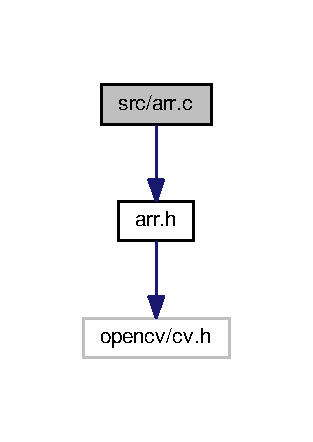
\includegraphics[width=150pt]{arr_8c__incl}
\end{center}
\end{figure}
\subsection*{Functions}
\begin{DoxyCompactItemize}
\item 
void \hyperlink{arr_8c_a1e06cf9c399bc46a3053d007b27d4b8a}{arr\-\_\-sub} (float $\ast$dst, float $\ast$src, size\-\_\-t size, float f)
\item 
void \hyperlink{arr_8c_a5a5edd40e86c7ab2dbc6a47eecad7e60}{arr\-\_\-add} (float dst\mbox{[}$\,$\mbox{]}, float src\mbox{[}$\,$\mbox{]}, size\-\_\-t size)
\item 
void \hyperlink{arr_8c_af4a473c67a36913419215a574e0d06eb}{arr\-\_\-abs} (float $\ast$dst, float $\ast$src, size\-\_\-t size)
\item 
float \hyperlink{arr_8c_a6c0fddffe790f7e4e09e3e2d283f3813}{arr\-\_\-sum} (float $\ast$arr, size\-\_\-t size)
\item 
size\-\_\-t \hyperlink{arr_8c_aabea581597f4de853707a7af358fc66c}{arr\-\_\-min\-\_\-idx} (const float $\ast$arr, size\-\_\-t size)
\item 
void \hyperlink{arr_8c_ae906b13d297231fed02b4c779d90a08b}{arr\-\_\-to\-\_\-\-Ipl\-Image} (Ipl\-Image $\ast$img, float $\ast$$\ast$arr, int height, int width, int channels)
\end{DoxyCompactItemize}


\subsection{Detailed Description}
Contains functions for handling array which are widely use in this program. \begin{DoxyAuthor}{Author}
Mathieu Fourcroy 
\end{DoxyAuthor}
\begin{DoxyDate}{Date}
07/15 
\end{DoxyDate}


\subsection{Function Documentation}
\hypertarget{arr_8c_af4a473c67a36913419215a574e0d06eb}{\index{arr.\-c@{arr.\-c}!arr\-\_\-abs@{arr\-\_\-abs}}
\index{arr\-\_\-abs@{arr\-\_\-abs}!arr.c@{arr.\-c}}
\subsubsection[{arr\-\_\-abs}]{\setlength{\rightskip}{0pt plus 5cm}void arr\-\_\-abs (
\begin{DoxyParamCaption}
\item[{float $\ast$}]{dst, }
\item[{float $\ast$}]{src, }
\item[{size\-\_\-t}]{size}
\end{DoxyParamCaption}
)}}\label{arr_8c_af4a473c67a36913419215a574e0d06eb}
Compute the absolute value of every elements of a given array.

\begin{DoxyNote}{Note}
The two arrays should have the same size which is 'size'.
\end{DoxyNote}

\begin{DoxyParams}[1]{Parameters}
\mbox{\tt out}  & {\em dst} & The array which will contains the result\-: the absolute values of 'src' elements.. \\
\hline
\mbox{\tt in}  & {\em src} & The initial array. \\
\hline
\mbox{\tt in}  & {\em size} & The size of the arrays. \\
\hline
\end{DoxyParams}


Here is the caller graph for this function\-:\nopagebreak
\begin{figure}[H]
\begin{center}
\leavevmode
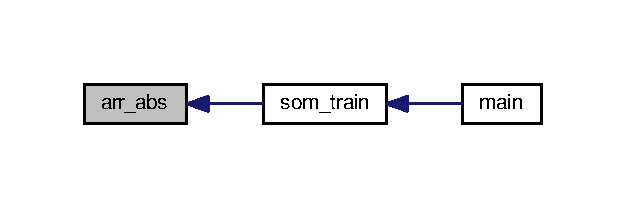
\includegraphics[width=300pt]{arr_8c_af4a473c67a36913419215a574e0d06eb_icgraph}
\end{center}
\end{figure}


\hypertarget{arr_8c_a5a5edd40e86c7ab2dbc6a47eecad7e60}{\index{arr.\-c@{arr.\-c}!arr\-\_\-add@{arr\-\_\-add}}
\index{arr\-\_\-add@{arr\-\_\-add}!arr.c@{arr.\-c}}
\subsubsection[{arr\-\_\-add}]{\setlength{\rightskip}{0pt plus 5cm}void arr\-\_\-add (
\begin{DoxyParamCaption}
\item[{float}]{dst\mbox{[}$\,$\mbox{]}, }
\item[{float}]{src\mbox{[}$\,$\mbox{]}, }
\item[{size\-\_\-t}]{size}
\end{DoxyParamCaption}
)}}\label{arr_8c_a5a5edd40e86c7ab2dbc6a47eecad7e60}
Compute the sum of two arrays.

\begin{DoxyWarning}{Warning}
The content of the 'dst' array will be modified to contains 'dst' + 'src'..
\end{DoxyWarning}
\begin{DoxyNote}{Note}
The two arrays should have the same size which is 'size'.
\end{DoxyNote}

\begin{DoxyParams}[1]{Parameters}
\mbox{\tt in,out}  & {\em dst} & The first array of the sum. It will contains the result. \\
\hline
\mbox{\tt in}  & {\em src} & The second array of the sum. \\
\hline
\mbox{\tt in}  & {\em size} & The size of the arrays. \\
\hline
\end{DoxyParams}


Here is the caller graph for this function\-:\nopagebreak
\begin{figure}[H]
\begin{center}
\leavevmode
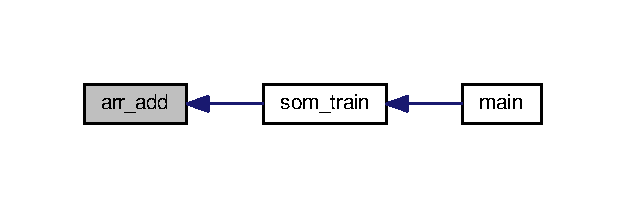
\includegraphics[width=300pt]{arr_8c_a5a5edd40e86c7ab2dbc6a47eecad7e60_icgraph}
\end{center}
\end{figure}


\hypertarget{arr_8c_aabea581597f4de853707a7af358fc66c}{\index{arr.\-c@{arr.\-c}!arr\-\_\-min\-\_\-idx@{arr\-\_\-min\-\_\-idx}}
\index{arr\-\_\-min\-\_\-idx@{arr\-\_\-min\-\_\-idx}!arr.c@{arr.\-c}}
\subsubsection[{arr\-\_\-min\-\_\-idx}]{\setlength{\rightskip}{0pt plus 5cm}size\-\_\-t arr\-\_\-min\-\_\-idx (
\begin{DoxyParamCaption}
\item[{const float $\ast$}]{arr, }
\item[{size\-\_\-t}]{size}
\end{DoxyParamCaption}
)}}\label{arr_8c_aabea581597f4de853707a7af358fc66c}
Find and returns the index of the minimum value in the given array.


\begin{DoxyParams}[1]{Parameters}
\mbox{\tt in}  & {\em arr} & The array. \\
\hline
\mbox{\tt in}  & {\em size} & The array size.\\
\hline
\end{DoxyParams}
\begin{DoxyReturn}{Returns}
The index of the lowest value of the array 'arr'. 
\end{DoxyReturn}


Here is the caller graph for this function\-:\nopagebreak
\begin{figure}[H]
\begin{center}
\leavevmode
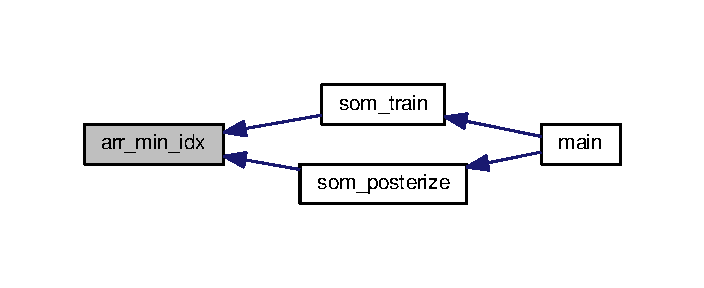
\includegraphics[width=338pt]{arr_8c_aabea581597f4de853707a7af358fc66c_icgraph}
\end{center}
\end{figure}


\hypertarget{arr_8c_a1e06cf9c399bc46a3053d007b27d4b8a}{\index{arr.\-c@{arr.\-c}!arr\-\_\-sub@{arr\-\_\-sub}}
\index{arr\-\_\-sub@{arr\-\_\-sub}!arr.c@{arr.\-c}}
\subsubsection[{arr\-\_\-sub}]{\setlength{\rightskip}{0pt plus 5cm}void arr\-\_\-sub (
\begin{DoxyParamCaption}
\item[{float $\ast$}]{dst, }
\item[{float $\ast$}]{src, }
\item[{size\-\_\-t}]{size, }
\item[{float}]{f}
\end{DoxyParamCaption}
)}}\label{arr_8c_a1e06cf9c399bc46a3053d007b27d4b8a}
Subtract a given float to every elements of a float array.


\begin{DoxyParams}[1]{Parameters}
\mbox{\tt out}  & {\em dst} & The destination array which will contains the resulting values. It must be of same size as 'src'. \\
\hline
\mbox{\tt in}  & {\em src} & The source array from which the results will be computed. \\
\hline
\mbox{\tt in}  & {\em size} & The size of the 'dst' and 'src' arrays. \\
\hline
\mbox{\tt in}  & {\em f} & The float number which will be subtract to every elements of the 'src' array. \\
\hline
\end{DoxyParams}


Here is the caller graph for this function\-:\nopagebreak
\begin{figure}[H]
\begin{center}
\leavevmode
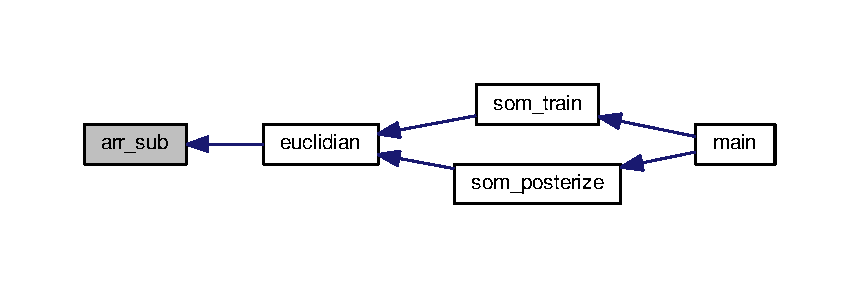
\includegraphics[width=350pt]{arr_8c_a1e06cf9c399bc46a3053d007b27d4b8a_icgraph}
\end{center}
\end{figure}


\hypertarget{arr_8c_a6c0fddffe790f7e4e09e3e2d283f3813}{\index{arr.\-c@{arr.\-c}!arr\-\_\-sum@{arr\-\_\-sum}}
\index{arr\-\_\-sum@{arr\-\_\-sum}!arr.c@{arr.\-c}}
\subsubsection[{arr\-\_\-sum}]{\setlength{\rightskip}{0pt plus 5cm}float arr\-\_\-sum (
\begin{DoxyParamCaption}
\item[{float $\ast$}]{arr, }
\item[{size\-\_\-t}]{size}
\end{DoxyParamCaption}
)}}\label{arr_8c_a6c0fddffe790f7e4e09e3e2d283f3813}
Compute and returns the sum of every elements of a given array.


\begin{DoxyParams}[1]{Parameters}
\mbox{\tt in}  & {\em arr} & The array to sum. \\
\hline
\mbox{\tt in}  & {\em size} & The size of the arrays.\\
\hline
\end{DoxyParams}
\begin{DoxyReturn}{Returns}
The sum of every elements of the given array of size 'size'. 
\end{DoxyReturn}


Here is the caller graph for this function\-:\nopagebreak
\begin{figure}[H]
\begin{center}
\leavevmode
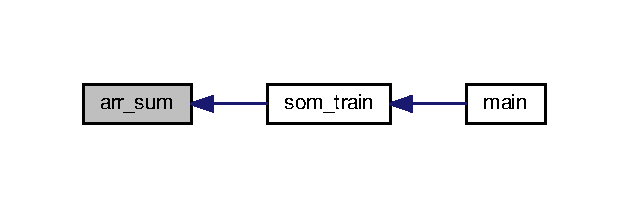
\includegraphics[width=302pt]{arr_8c_a6c0fddffe790f7e4e09e3e2d283f3813_icgraph}
\end{center}
\end{figure}


\hypertarget{arr_8c_ae906b13d297231fed02b4c779d90a08b}{\index{arr.\-c@{arr.\-c}!arr\-\_\-to\-\_\-\-Ipl\-Image@{arr\-\_\-to\-\_\-\-Ipl\-Image}}
\index{arr\-\_\-to\-\_\-\-Ipl\-Image@{arr\-\_\-to\-\_\-\-Ipl\-Image}!arr.c@{arr.\-c}}
\subsubsection[{arr\-\_\-to\-\_\-\-Ipl\-Image}]{\setlength{\rightskip}{0pt plus 5cm}void arr\-\_\-to\-\_\-\-Ipl\-Image (
\begin{DoxyParamCaption}
\item[{Ipl\-Image $\ast$}]{img, }
\item[{float $\ast$$\ast$}]{arr, }
\item[{int}]{height, }
\item[{int}]{width, }
\item[{int}]{channels}
\end{DoxyParamCaption}
)}}\label{arr_8c_ae906b13d297231fed02b4c779d90a08b}
Flatten a 2\-D array and modify the given image data.


\begin{DoxyParams}[1]{Parameters}
\mbox{\tt in,out}  & {\em img} & The image wich will be modified with the data of 'arr'. \\
\hline
\mbox{\tt in}  & {\em arr} & The 2\-D array containing the posterized pixels. \\
\hline
\mbox{\tt in}  & {\em height} & The image height. \\
\hline
\mbox{\tt in}  & {\em width} & The image width. \\
\hline
\mbox{\tt in}  & {\em channels} & The number of channels of the image. \\
\hline
\end{DoxyParams}


Here is the caller graph for this function\-:\nopagebreak
\begin{figure}[H]
\begin{center}
\leavevmode
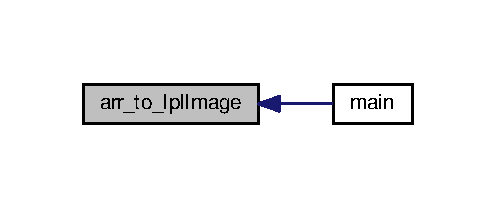
\includegraphics[width=238pt]{arr_8c_ae906b13d297231fed02b4c779d90a08b_icgraph}
\end{center}
\end{figure}



\hypertarget{arr_8h}{\section{src/arr.h File Reference}
\label{arr_8h}\index{src/arr.\-h@{src/arr.\-h}}
}
{\ttfamily \#include $<$opencv/cv.\-h$>$}\\*
Include dependency graph for arr.\-h\-:\nopagebreak
\begin{figure}[H]
\begin{center}
\leavevmode
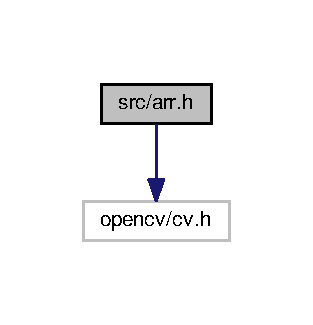
\includegraphics[width=150pt]{arr_8h__incl}
\end{center}
\end{figure}
This graph shows which files directly or indirectly include this file\-:\nopagebreak
\begin{figure}[H]
\begin{center}
\leavevmode
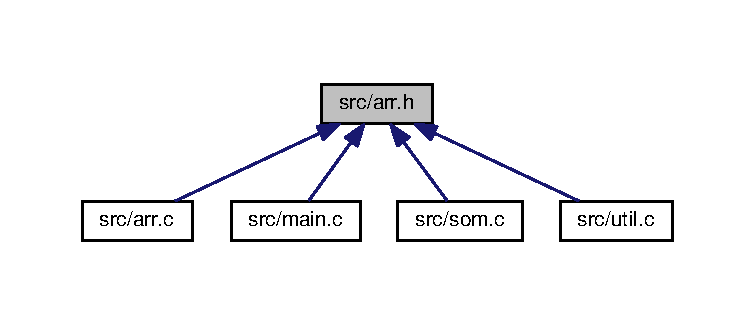
\includegraphics[width=350pt]{arr_8h__dep__incl}
\end{center}
\end{figure}
\subsection*{Functions}
\begin{DoxyCompactItemize}
\item 
void \hyperlink{arr_8h_a1e06cf9c399bc46a3053d007b27d4b8a}{arr\-\_\-sub} (float $\ast$dst, float $\ast$src, size\-\_\-t size, float f)
\item 
void \hyperlink{arr_8h_a5a5edd40e86c7ab2dbc6a47eecad7e60}{arr\-\_\-add} (float dst\mbox{[}$\,$\mbox{]}, float src\mbox{[}$\,$\mbox{]}, size\-\_\-t size)
\item 
void \hyperlink{arr_8h_af4a473c67a36913419215a574e0d06eb}{arr\-\_\-abs} (float $\ast$dst, float $\ast$src, size\-\_\-t size)
\item 
float \hyperlink{arr_8h_a6c0fddffe790f7e4e09e3e2d283f3813}{arr\-\_\-sum} (float $\ast$arr, size\-\_\-t size)
\item 
size\-\_\-t \hyperlink{arr_8h_aabea581597f4de853707a7af358fc66c}{arr\-\_\-min\-\_\-idx} (const float $\ast$arr, size\-\_\-t size)
\item 
void \hyperlink{arr_8h_ae906b13d297231fed02b4c779d90a08b}{arr\-\_\-to\-\_\-\-Ipl\-Image} (Ipl\-Image $\ast$img, float $\ast$$\ast$arr, int height, int width, int channels)
\end{DoxyCompactItemize}


\subsection{Function Documentation}
\hypertarget{arr_8h_af4a473c67a36913419215a574e0d06eb}{\index{arr.\-h@{arr.\-h}!arr\-\_\-abs@{arr\-\_\-abs}}
\index{arr\-\_\-abs@{arr\-\_\-abs}!arr.h@{arr.\-h}}
\subsubsection[{arr\-\_\-abs}]{\setlength{\rightskip}{0pt plus 5cm}void arr\-\_\-abs (
\begin{DoxyParamCaption}
\item[{float $\ast$}]{dst, }
\item[{float $\ast$}]{src, }
\item[{size\-\_\-t}]{size}
\end{DoxyParamCaption}
)}}\label{arr_8h_af4a473c67a36913419215a574e0d06eb}
Compute the absolute value of every elements of a given array.

\begin{DoxyNote}{Note}
The two arrays should have the same size which is 'size'.
\end{DoxyNote}

\begin{DoxyParams}[1]{Parameters}
\mbox{\tt out}  & {\em dst} & The array which will contains the result\-: the absolute values of 'src' elements.. \\
\hline
\mbox{\tt in}  & {\em src} & The initial array. \\
\hline
\mbox{\tt in}  & {\em size} & The size of the arrays. \\
\hline
\end{DoxyParams}


Here is the caller graph for this function\-:\nopagebreak
\begin{figure}[H]
\begin{center}
\leavevmode
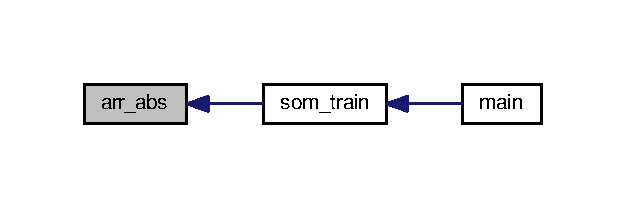
\includegraphics[width=300pt]{arr_8h_af4a473c67a36913419215a574e0d06eb_icgraph}
\end{center}
\end{figure}


\hypertarget{arr_8h_a5a5edd40e86c7ab2dbc6a47eecad7e60}{\index{arr.\-h@{arr.\-h}!arr\-\_\-add@{arr\-\_\-add}}
\index{arr\-\_\-add@{arr\-\_\-add}!arr.h@{arr.\-h}}
\subsubsection[{arr\-\_\-add}]{\setlength{\rightskip}{0pt plus 5cm}void arr\-\_\-add (
\begin{DoxyParamCaption}
\item[{float}]{dst\mbox{[}$\,$\mbox{]}, }
\item[{float}]{src\mbox{[}$\,$\mbox{]}, }
\item[{size\-\_\-t}]{size}
\end{DoxyParamCaption}
)}}\label{arr_8h_a5a5edd40e86c7ab2dbc6a47eecad7e60}
Compute the sum of two arrays.

\begin{DoxyWarning}{Warning}
The content of the 'dst' array will be modified to contains 'dst' + 'src'..
\end{DoxyWarning}
\begin{DoxyNote}{Note}
The two arrays should have the same size which is 'size'.
\end{DoxyNote}

\begin{DoxyParams}[1]{Parameters}
\mbox{\tt in,out}  & {\em dst} & The first array of the sum. It will contains the result. \\
\hline
\mbox{\tt in}  & {\em src} & The second array of the sum. \\
\hline
\mbox{\tt in}  & {\em size} & The size of the arrays. \\
\hline
\end{DoxyParams}


Here is the caller graph for this function\-:\nopagebreak
\begin{figure}[H]
\begin{center}
\leavevmode
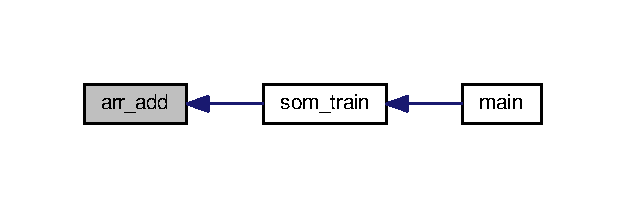
\includegraphics[width=300pt]{arr_8h_a5a5edd40e86c7ab2dbc6a47eecad7e60_icgraph}
\end{center}
\end{figure}


\hypertarget{arr_8h_aabea581597f4de853707a7af358fc66c}{\index{arr.\-h@{arr.\-h}!arr\-\_\-min\-\_\-idx@{arr\-\_\-min\-\_\-idx}}
\index{arr\-\_\-min\-\_\-idx@{arr\-\_\-min\-\_\-idx}!arr.h@{arr.\-h}}
\subsubsection[{arr\-\_\-min\-\_\-idx}]{\setlength{\rightskip}{0pt plus 5cm}size\-\_\-t arr\-\_\-min\-\_\-idx (
\begin{DoxyParamCaption}
\item[{const float $\ast$}]{arr, }
\item[{size\-\_\-t}]{size}
\end{DoxyParamCaption}
)}}\label{arr_8h_aabea581597f4de853707a7af358fc66c}
Find and returns the index of the minimum value in the given array.


\begin{DoxyParams}[1]{Parameters}
\mbox{\tt in}  & {\em arr} & The array. \\
\hline
\mbox{\tt in}  & {\em size} & The array size.\\
\hline
\end{DoxyParams}
\begin{DoxyReturn}{Returns}
The index of the lowest value of the array 'arr'. 
\end{DoxyReturn}


Here is the caller graph for this function\-:\nopagebreak
\begin{figure}[H]
\begin{center}
\leavevmode
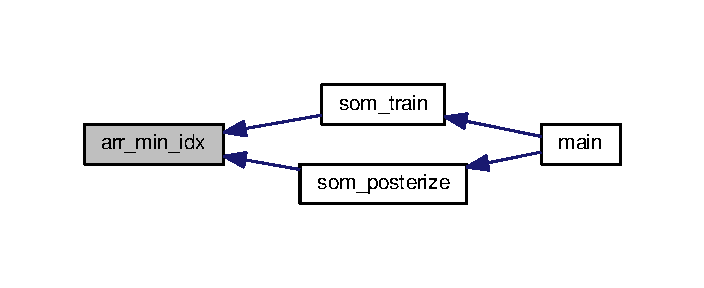
\includegraphics[width=338pt]{arr_8h_aabea581597f4de853707a7af358fc66c_icgraph}
\end{center}
\end{figure}


\hypertarget{arr_8h_a1e06cf9c399bc46a3053d007b27d4b8a}{\index{arr.\-h@{arr.\-h}!arr\-\_\-sub@{arr\-\_\-sub}}
\index{arr\-\_\-sub@{arr\-\_\-sub}!arr.h@{arr.\-h}}
\subsubsection[{arr\-\_\-sub}]{\setlength{\rightskip}{0pt plus 5cm}void arr\-\_\-sub (
\begin{DoxyParamCaption}
\item[{float $\ast$}]{dst, }
\item[{float $\ast$}]{src, }
\item[{size\-\_\-t}]{size, }
\item[{float}]{f}
\end{DoxyParamCaption}
)}}\label{arr_8h_a1e06cf9c399bc46a3053d007b27d4b8a}
Subtract a given float to every elements of a float array.


\begin{DoxyParams}[1]{Parameters}
\mbox{\tt out}  & {\em dst} & The destination array which will contains the resulting values. It must be of same size as 'src'. \\
\hline
\mbox{\tt in}  & {\em src} & The source array from which the results will be computed. \\
\hline
\mbox{\tt in}  & {\em size} & The size of the 'dst' and 'src' arrays. \\
\hline
\mbox{\tt in}  & {\em f} & The float number which will be subtract to every elements of the 'src' array. \\
\hline
\end{DoxyParams}


Here is the caller graph for this function\-:\nopagebreak
\begin{figure}[H]
\begin{center}
\leavevmode
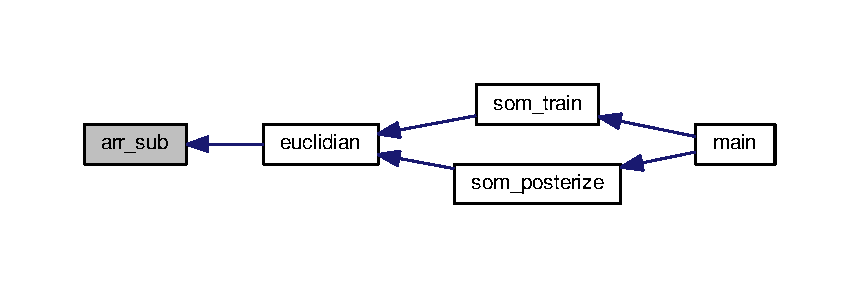
\includegraphics[width=350pt]{arr_8h_a1e06cf9c399bc46a3053d007b27d4b8a_icgraph}
\end{center}
\end{figure}


\hypertarget{arr_8h_a6c0fddffe790f7e4e09e3e2d283f3813}{\index{arr.\-h@{arr.\-h}!arr\-\_\-sum@{arr\-\_\-sum}}
\index{arr\-\_\-sum@{arr\-\_\-sum}!arr.h@{arr.\-h}}
\subsubsection[{arr\-\_\-sum}]{\setlength{\rightskip}{0pt plus 5cm}float arr\-\_\-sum (
\begin{DoxyParamCaption}
\item[{float $\ast$}]{arr, }
\item[{size\-\_\-t}]{size}
\end{DoxyParamCaption}
)}}\label{arr_8h_a6c0fddffe790f7e4e09e3e2d283f3813}
Compute and returns the sum of every elements of a given array.


\begin{DoxyParams}[1]{Parameters}
\mbox{\tt in}  & {\em arr} & The array to sum. \\
\hline
\mbox{\tt in}  & {\em size} & The size of the arrays.\\
\hline
\end{DoxyParams}
\begin{DoxyReturn}{Returns}
The sum of every elements of the given array of size 'size'. 
\end{DoxyReturn}


Here is the caller graph for this function\-:\nopagebreak
\begin{figure}[H]
\begin{center}
\leavevmode
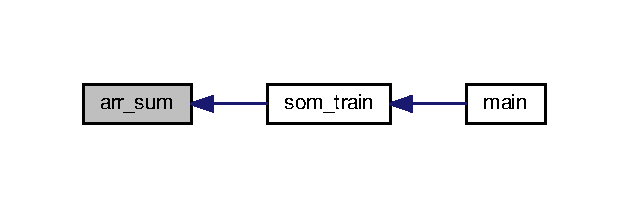
\includegraphics[width=302pt]{arr_8h_a6c0fddffe790f7e4e09e3e2d283f3813_icgraph}
\end{center}
\end{figure}


\hypertarget{arr_8h_ae906b13d297231fed02b4c779d90a08b}{\index{arr.\-h@{arr.\-h}!arr\-\_\-to\-\_\-\-Ipl\-Image@{arr\-\_\-to\-\_\-\-Ipl\-Image}}
\index{arr\-\_\-to\-\_\-\-Ipl\-Image@{arr\-\_\-to\-\_\-\-Ipl\-Image}!arr.h@{arr.\-h}}
\subsubsection[{arr\-\_\-to\-\_\-\-Ipl\-Image}]{\setlength{\rightskip}{0pt plus 5cm}void arr\-\_\-to\-\_\-\-Ipl\-Image (
\begin{DoxyParamCaption}
\item[{Ipl\-Image $\ast$}]{img, }
\item[{float $\ast$$\ast$}]{arr, }
\item[{int}]{height, }
\item[{int}]{width, }
\item[{int}]{channels}
\end{DoxyParamCaption}
)}}\label{arr_8h_ae906b13d297231fed02b4c779d90a08b}
Flatten a 2\-D array and modify the given image data.


\begin{DoxyParams}[1]{Parameters}
\mbox{\tt in,out}  & {\em img} & The image wich will be modified with the data of 'arr'. \\
\hline
\mbox{\tt in}  & {\em arr} & The 2\-D array containing the posterized pixels. \\
\hline
\mbox{\tt in}  & {\em height} & The image height. \\
\hline
\mbox{\tt in}  & {\em width} & The image width. \\
\hline
\mbox{\tt in}  & {\em channels} & The number of channels of the image. \\
\hline
\end{DoxyParams}


Here is the caller graph for this function\-:\nopagebreak
\begin{figure}[H]
\begin{center}
\leavevmode
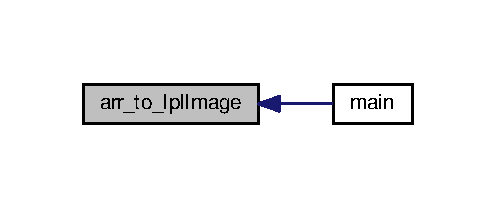
\includegraphics[width=238pt]{arr_8h_ae906b13d297231fed02b4c779d90a08b_icgraph}
\end{center}
\end{figure}



\hypertarget{main_8c}{\section{src/main.c File Reference}
\label{main_8c}\index{src/main.\-c@{src/main.\-c}}
}


Main file of the program. Take care of I/\-O and call the other functions.  


{\ttfamily \#include $<$opencv/highgui.\-h$>$}\\*
{\ttfamily \#include $<$stdio.\-h$>$}\\*
{\ttfamily \#include $<$ctype.\-h$>$}\\*
{\ttfamily \#include $<$getopt.\-h$>$}\\*
{\ttfamily \#include \char`\"{}arr.\-h\char`\"{}}\\*
{\ttfamily \#include \char`\"{}som.\-h\char`\"{}}\\*
{\ttfamily \#include \char`\"{}util.\-h\char`\"{}}\\*
Include dependency graph for main.\-c\-:\nopagebreak
\begin{figure}[H]
\begin{center}
\leavevmode
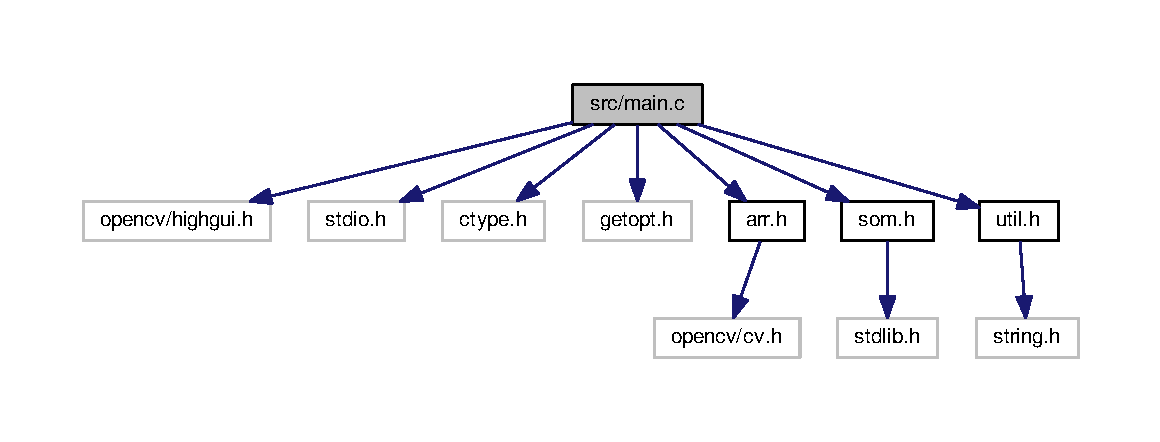
\includegraphics[width=350pt]{main_8c__incl}
\end{center}
\end{figure}
\subsection*{Functions}
\begin{DoxyCompactItemize}
\item 
void \hyperlink{main_8c_ae8605e2b78cd4a81b6c6b5c30cb7366a}{usage} (void)
\item 
int \hyperlink{main_8c_a8a30a7c1d99382d3d205b4c924e3dd18}{set\-\_\-vars\-\_\-from\-\_\-args} (int argc, char $\ast$const argv\mbox{[}$\,$\mbox{]}, int $\ast$post\-Level, int $\ast$epochs, float $\ast$thresh, char $\ast$in\-File, char $\ast$out\-File)
\item 
int \hyperlink{main_8c_af3ed9c200de85b53c94cd18764b246a2}{main} (int argc, char $\ast$const argv\mbox{[}$\,$\mbox{]})
\end{DoxyCompactItemize}


\subsection{Detailed Description}
Main file of the program. Take care of I/\-O and call the other functions. \begin{DoxyAuthor}{Author}
Mathieu Fourcroy 
\end{DoxyAuthor}
\begin{DoxyDate}{Date}
07/15 
\end{DoxyDate}


\subsection{Function Documentation}
\hypertarget{main_8c_af3ed9c200de85b53c94cd18764b246a2}{\index{main.\-c@{main.\-c}!main@{main}}
\index{main@{main}!main.c@{main.\-c}}
\subsubsection[{main}]{\setlength{\rightskip}{0pt plus 5cm}int main (
\begin{DoxyParamCaption}
\item[{int}]{argc, }
\item[{char $\ast$const}]{argv\mbox{[}$\,$\mbox{]}}
\end{DoxyParamCaption}
)}}\label{main_8c_af3ed9c200de85b53c94cd18764b246a2}
The main function

The main function scan the command line and set the program variables using the specified options or the default values. Then The function open the image from the input path and load it. Its pixels are extracted. The S\-O\-M network is trained from random values and using the image pixels. The S\-O\-M resulting neurons represent the colors used for the posterization. So the posterization function use the result of the S\-O\-M network to effectively posterized the image. The image pixels are directly modified. Finaly the modified image is saved as a new file.

\begin{DoxyNote}{Note}
The number of neurons of the network is the posterization level power two. Which means that the S\-O\-M is square. It has a number of rows and a number of columns equal to the posterization level. So it have rows $\ast$ columns = rows$^\wedge$2 = columns$^\wedge$2 = posterization level$^\wedge$2 = number of neurons.
\end{DoxyNote}
\begin{DoxyWarning}{Warning}
The transparency in file formats which support it is not correctly handled.
\end{DoxyWarning}
\begin{DoxyRefDesc}{Todo}
\item[\hyperlink{todo__todo000001}{Todo}]0.\-0.\-2 Handle transparency with opencv and the S\-O\-M algorithm. The program currently use the number of channels of the image but it is always 3 (R\-G\-B) for now. \end{DoxyRefDesc}


Here is the call graph for this function\-:\nopagebreak
\begin{figure}[H]
\begin{center}
\leavevmode
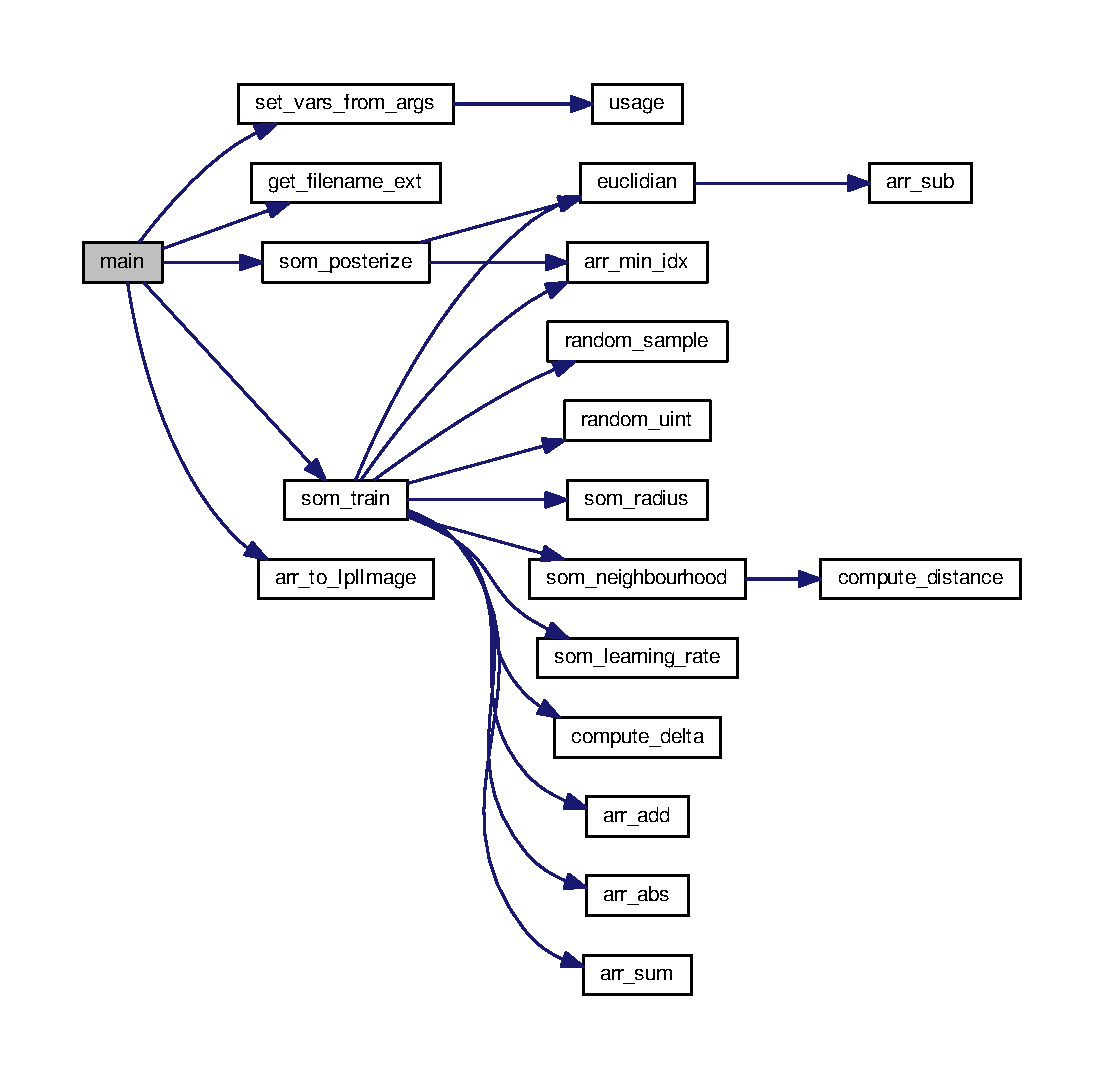
\includegraphics[width=350pt]{main_8c_af3ed9c200de85b53c94cd18764b246a2_cgraph}
\end{center}
\end{figure}


\hypertarget{main_8c_a8a30a7c1d99382d3d205b4c924e3dd18}{\index{main.\-c@{main.\-c}!set\-\_\-vars\-\_\-from\-\_\-args@{set\-\_\-vars\-\_\-from\-\_\-args}}
\index{set\-\_\-vars\-\_\-from\-\_\-args@{set\-\_\-vars\-\_\-from\-\_\-args}!main.c@{main.\-c}}
\subsubsection[{set\-\_\-vars\-\_\-from\-\_\-args}]{\setlength{\rightskip}{0pt plus 5cm}int set\-\_\-vars\-\_\-from\-\_\-args (
\begin{DoxyParamCaption}
\item[{int}]{argc, }
\item[{char $\ast$const}]{argv\mbox{[}$\,$\mbox{]}, }
\item[{int $\ast$}]{post\-Level, }
\item[{int $\ast$}]{epochs, }
\item[{float $\ast$}]{thresh, }
\item[{char $\ast$}]{in\-File, }
\item[{char $\ast$}]{out\-File}
\end{DoxyParamCaption}
)}}\label{main_8c_a8a30a7c1d99382d3d205b4c924e3dd18}
Parse the options from the command line.


\begin{DoxyParams}[1]{Parameters}
\mbox{\tt in}  & {\em argc} & Number of arguments on the command line. \\
\hline
\mbox{\tt in}  & {\em argv} & The arguments of the command line. \\
\hline
\mbox{\tt out}  & {\em post\-Level} & Posterization level (set by -\/l / default\-: 2). \\
\hline
\mbox{\tt out}  & {\em epochs} & Number of training stage (set by -\/e / default\-: 3000). \\
\hline
\mbox{\tt out}  & {\em thresh} & Network threshold value (set by -\/t / default\-: 0.\-001). \\
\hline
\mbox{\tt out}  & {\em in\-File} & Path to the input image (must be set with -\/i). \\
\hline
\mbox{\tt out}  & {\em out\-File} & Path to the output image (set by -\/o). \\
\hline
\end{DoxyParams}


Here is the call graph for this function\-:\nopagebreak
\begin{figure}[H]
\begin{center}
\leavevmode
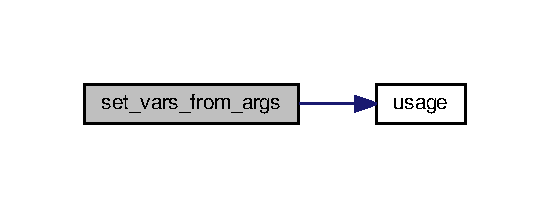
\includegraphics[width=264pt]{main_8c_a8a30a7c1d99382d3d205b4c924e3dd18_cgraph}
\end{center}
\end{figure}




Here is the caller graph for this function\-:\nopagebreak
\begin{figure}[H]
\begin{center}
\leavevmode
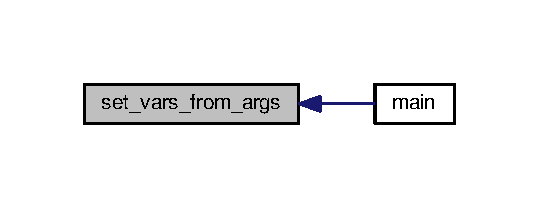
\includegraphics[width=258pt]{main_8c_a8a30a7c1d99382d3d205b4c924e3dd18_icgraph}
\end{center}
\end{figure}


\hypertarget{main_8c_ae8605e2b78cd4a81b6c6b5c30cb7366a}{\index{main.\-c@{main.\-c}!usage@{usage}}
\index{usage@{usage}!main.c@{main.\-c}}
\subsubsection[{usage}]{\setlength{\rightskip}{0pt plus 5cm}void usage (
\begin{DoxyParamCaption}
\item[{void}]{}
\end{DoxyParamCaption}
)}}\label{main_8c_ae8605e2b78cd4a81b6c6b5c30cb7366a}
Print a usage message. 

Here is the caller graph for this function\-:\nopagebreak
\begin{figure}[H]
\begin{center}
\leavevmode
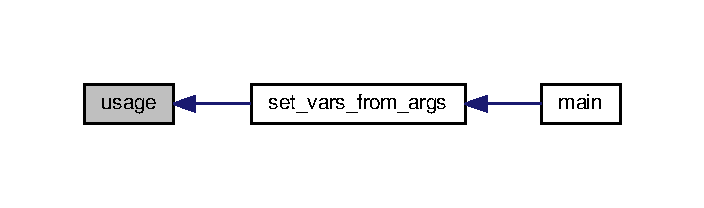
\includegraphics[width=338pt]{main_8c_ae8605e2b78cd4a81b6c6b5c30cb7366a_icgraph}
\end{center}
\end{figure}



\hypertarget{mainpage_8dox}{\section{src/mainpage.dox File Reference}
\label{mainpage_8dox}\index{src/mainpage.\-dox@{src/mainpage.\-dox}}
}

\hypertarget{som_8c}{\section{src/som.c File Reference}
\label{som_8c}\index{src/som.\-c@{src/som.\-c}}
}


Contains functions about the self organized map neural network implemented for the project.  


{\ttfamily \#include $<$string.\-h$>$}\\*
{\ttfamily \#include $<$time.\-h$>$}\\*
{\ttfamily \#include $<$math.\-h$>$}\\*
{\ttfamily \#include $<$limits.\-h$>$}\\*
{\ttfamily \#include \char`\"{}som.\-h\char`\"{}}\\*
{\ttfamily \#include \char`\"{}arr.\-h\char`\"{}}\\*
{\ttfamily \#include \char`\"{}util.\-h\char`\"{}}\\*
Include dependency graph for som.\-c\-:\nopagebreak
\begin{figure}[H]
\begin{center}
\leavevmode
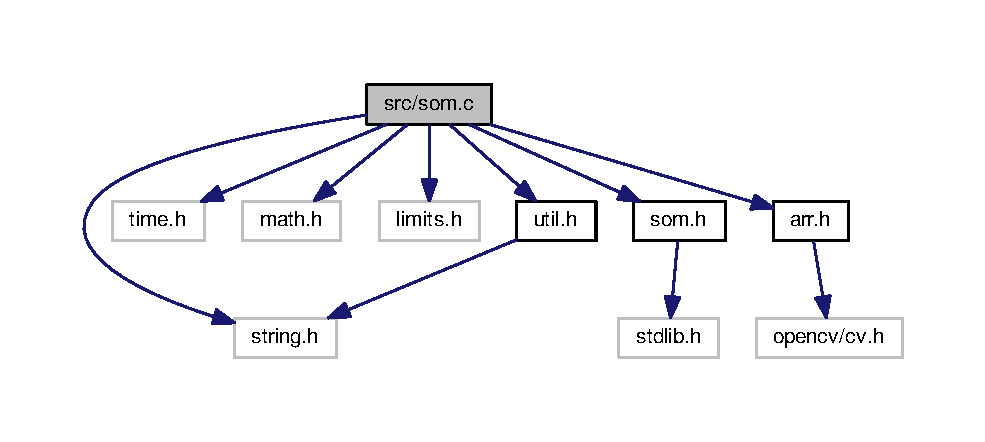
\includegraphics[width=350pt]{som_8c__incl}
\end{center}
\end{figure}
\subsection*{Functions}
\begin{DoxyCompactItemize}
\item 
static float \hyperlink{som_8c_a577de332dd926969d02e86228f65ad8f}{som\-\_\-radius} (int iter\-No, int iter\-Count, int width, int height)
\item 
static float \hyperlink{som_8c_ad269dc9f88dff13ec50497edc5bde2b0}{som\-\_\-learning\-\_\-rate} (int iter\-No, int iter\-Count)
\item 
static int \hyperlink{som_8c_a299abea75e13175cea5a3dbe748c65a1}{euclidian} (float $\ast$res, size\-\_\-t size, float $\ast$x, float $\ast$y, float $\ast$z, float $\ast$R\-G\-B)
\item 
static float \hyperlink{som_8c_a1b36e26588b00c18c3b967366b63bca4}{compute\-\_\-distance} (int i, int y, int j, int x)
\item 
static void \hyperlink{som_8c_a1603f0fc083688b151b2ad414f9120a5}{som\-\_\-neighbourhood} (float $\ast$neigh, int x, int y, float radius, int width, int height)
\item 
void \hyperlink{som_8c_a392441531c1d2025232854783e7014bf}{compute\-\_\-delta} (float $\ast$res, float eta, float $\ast$neigh, size\-\_\-t nb\-Neigh, float chan, float $\ast$chan\-Arr)
\item 
int \hyperlink{som_8c_ab268269d2bda7d28482c0627e7c102ab}{som\-\_\-train} (float $\ast$$\ast$res, float $\ast$$\ast$img\-Pixels, unsigned int nb\-Pixels, int nb\-Neurons, int no\-Epoch, float thresh)
\item 
void \hyperlink{som_8c_a3e18491e97ad6c14f54ba35aabfab994}{som\-\_\-posterize} (float $\ast$$\ast$post\-Pixels, float $\ast$$\ast$orig\-Pixels, float $\ast$train\mbox{[}$\,$\mbox{]}, unsigned int nb\-Pixels, int nb\-Neurons)
\end{DoxyCompactItemize}


\subsection{Detailed Description}
Contains functions about the self organized map neural network implemented for the project. \begin{DoxyAuthor}{Author}
Mathieu Fourcroy 
\end{DoxyAuthor}
\begin{DoxyDate}{Date}
07/15 
\end{DoxyDate}


\subsection{Function Documentation}
\hypertarget{som_8c_a392441531c1d2025232854783e7014bf}{\index{som.\-c@{som.\-c}!compute\-\_\-delta@{compute\-\_\-delta}}
\index{compute\-\_\-delta@{compute\-\_\-delta}!som.c@{som.\-c}}
\subsubsection[{compute\-\_\-delta}]{\setlength{\rightskip}{0pt plus 5cm}void compute\-\_\-delta (
\begin{DoxyParamCaption}
\item[{float $\ast$}]{res, }
\item[{float}]{eta, }
\item[{float $\ast$}]{neigh, }
\item[{size\-\_\-t}]{nb\-Neigh, }
\item[{float}]{chan, }
\item[{float $\ast$}]{chan\-Arr}
\end{DoxyParamCaption}
)}}\label{som_8c_a392441531c1d2025232854783e7014bf}
Compute the new neurons values (learning stage).

This function compute the new neurons values depending on the learning rate (eta), the winner neighboors (neigh) and the choosed input vector (chan). The network wieght vectors inside the neighbooring radius are modified so that they will be more similar to the choosen input vector.


\begin{DoxyParams}[1]{Parameters}
\mbox{\tt out}  & {\em res} & The resulting array containing the delta values. \\
\hline
\mbox{\tt in}  & {\em eta} & The learning rate. \\
\hline
\mbox{\tt in}  & {\em neigh} & Array listing the current neighbors of the network. \\
\hline
\mbox{\tt in}  & {\em nb\-Neigh} & The size of the \char`\"{}neigh\char`\"{} array. \\
\hline
\mbox{\tt in}  & {\em chan} & The value of the color channel. \\
\hline
\mbox{\tt in}  & {\em chan\-Arr} & The array corresponding to the given channel. \\
\hline
\end{DoxyParams}


Here is the caller graph for this function\-:\nopagebreak
\begin{figure}[H]
\begin{center}
\leavevmode
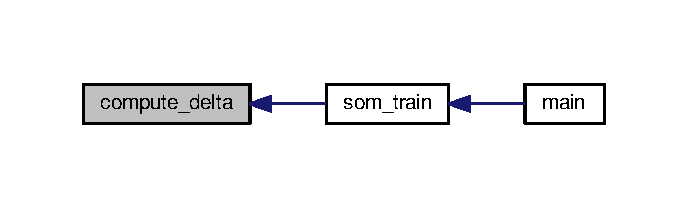
\includegraphics[width=330pt]{som_8c_a392441531c1d2025232854783e7014bf_icgraph}
\end{center}
\end{figure}


\hypertarget{som_8c_a1b36e26588b00c18c3b967366b63bca4}{\index{som.\-c@{som.\-c}!compute\-\_\-distance@{compute\-\_\-distance}}
\index{compute\-\_\-distance@{compute\-\_\-distance}!som.c@{som.\-c}}
\subsubsection[{compute\-\_\-distance}]{\setlength{\rightskip}{0pt plus 5cm}static float compute\-\_\-distance (
\begin{DoxyParamCaption}
\item[{int}]{i, }
\item[{int}]{y, }
\item[{int}]{j, }
\item[{int}]{x}
\end{DoxyParamCaption}
)\hspace{0.3cm}{\ttfamily [static]}}}\label{som_8c_a1b36e26588b00c18c3b967366b63bca4}
Compute the euclidian distance between two 2\-D points.

\begin{DoxySeeAlso}{See Also}
\href{https://en.wikipedia.org/wiki/Euclidean_distance}{\tt https\-://en.\-wikipedia.\-org/wiki/\-Euclidean\-\_\-distance}
\end{DoxySeeAlso}

\begin{DoxyParams}[1]{Parameters}
\mbox{\tt in}  & {\em i} & The first point abscissae. \\
\hline
\mbox{\tt in}  & {\em y} & The first point ordinates. \\
\hline
\mbox{\tt in}  & {\em j} & The second point abscissae. \\
\hline
\mbox{\tt in}  & {\em x} & The second point ordinates.\\
\hline
\end{DoxyParams}
\begin{DoxyReturn}{Returns}
The euclidian distance between the points (i, j) and (y, x). 
\end{DoxyReturn}


Here is the caller graph for this function\-:\nopagebreak
\begin{figure}[H]
\begin{center}
\leavevmode
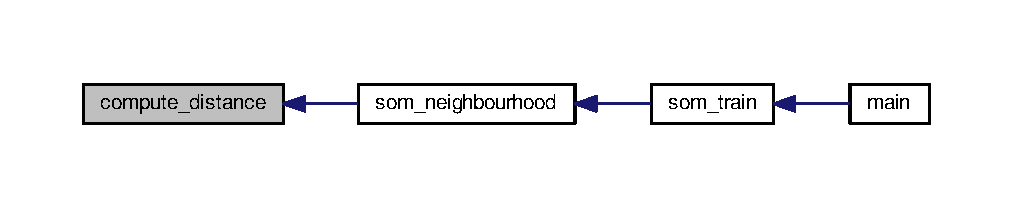
\includegraphics[width=350pt]{som_8c_a1b36e26588b00c18c3b967366b63bca4_icgraph}
\end{center}
\end{figure}


\hypertarget{som_8c_a299abea75e13175cea5a3dbe748c65a1}{\index{som.\-c@{som.\-c}!euclidian@{euclidian}}
\index{euclidian@{euclidian}!som.c@{som.\-c}}
\subsubsection[{euclidian}]{\setlength{\rightskip}{0pt plus 5cm}static int euclidian (
\begin{DoxyParamCaption}
\item[{float $\ast$}]{res, }
\item[{size\-\_\-t}]{size, }
\item[{float $\ast$}]{x, }
\item[{float $\ast$}]{y, }
\item[{float $\ast$}]{z, }
\item[{float $\ast$}]{R\-G\-B}
\end{DoxyParamCaption}
)\hspace{0.3cm}{\ttfamily [static]}}}\label{som_8c_a299abea75e13175cea5a3dbe748c65a1}
Compute the Euclidian distance between weight vectors and input vector.

The Euclidean distance between points p and q is the length of the line segment connecting them.

\begin{DoxySeeAlso}{See Also}
\href{https://en.wikipedia.org/wiki/Euclidean_distance}{\tt https\-://en.\-wikipedia.\-org/wiki/\-Euclidean\-\_\-distance}.
\end{DoxySeeAlso}
The two points here are (x, y, z) and (R\-G\-B\mbox{[}0\mbox{]}, R\-G\-B\mbox{[}1\mbox{]}, R\-G\-B\mbox{[}2\mbox{]}).


\begin{DoxyParams}[1]{Parameters}
\mbox{\tt out}  & {\em res} & The array which will contain the euclidian distance. It must be of size 'size'. \\
\hline
\mbox{\tt in}  & {\em size} & Size of the 'x', 'y', 'z' and 'res' arrays. \\
\hline
\mbox{\tt in}  & {\em x} & The x 3\-D coordinates. \\
\hline
\mbox{\tt in}  & {\em y} & The y 3\-D coordinates. \\
\hline
\mbox{\tt in}  & {\em z} & The z 3\-D coordinates. \\
\hline
\mbox{\tt in}  & {\em R\-G\-B} & The array containing the three channels values, treated as coordinates.\\
\hline
\end{DoxyParams}
\begin{DoxyReturn}{Returns}
S\-O\-M\-\_\-\-O\-K if everything goes right or S\-O\-M\-\_\-\-N\-O\-\_\-\-M\-E\-M\-O\-R\-Y if a memory allocation (malloc) fail. 
\end{DoxyReturn}


Here is the call graph for this function\-:\nopagebreak
\begin{figure}[H]
\begin{center}
\leavevmode
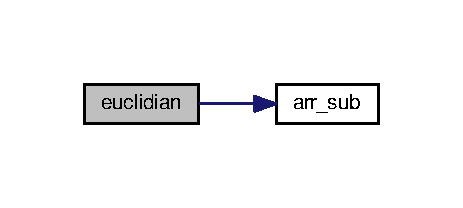
\includegraphics[width=222pt]{som_8c_a299abea75e13175cea5a3dbe748c65a1_cgraph}
\end{center}
\end{figure}




Here is the caller graph for this function\-:\nopagebreak
\begin{figure}[H]
\begin{center}
\leavevmode
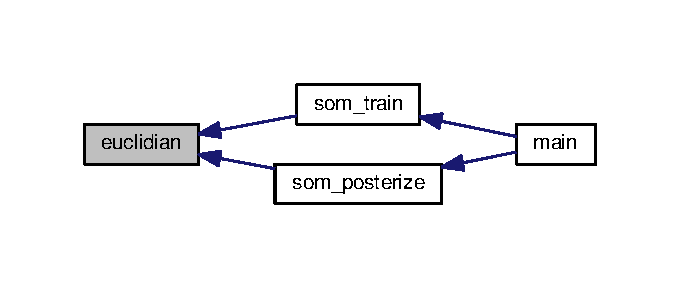
\includegraphics[width=326pt]{som_8c_a299abea75e13175cea5a3dbe748c65a1_icgraph}
\end{center}
\end{figure}


\hypertarget{som_8c_ad269dc9f88dff13ec50497edc5bde2b0}{\index{som.\-c@{som.\-c}!som\-\_\-learning\-\_\-rate@{som\-\_\-learning\-\_\-rate}}
\index{som\-\_\-learning\-\_\-rate@{som\-\_\-learning\-\_\-rate}!som.c@{som.\-c}}
\subsubsection[{som\-\_\-learning\-\_\-rate}]{\setlength{\rightskip}{0pt plus 5cm}static float som\-\_\-learning\-\_\-rate (
\begin{DoxyParamCaption}
\item[{int}]{iter\-No, }
\item[{int}]{iter\-Count}
\end{DoxyParamCaption}
)\hspace{0.3cm}{\ttfamily [static]}}}\label{som_8c_ad269dc9f88dff13ec50497edc5bde2b0}
Compute and returns the learning rate of the network.

The learning rate is a function of the current iteration number over the maximum iterations number and a given range.


\begin{DoxyParams}[1]{Parameters}
\mbox{\tt in}  & {\em iter\-No} & The number of the current iteration. \\
\hline
\mbox{\tt in}  & {\em iter\-Count} & The maximum number of iterations.\\
\hline
\end{DoxyParams}
\begin{DoxyReturn}{Returns}
The computed learning rate. 
\end{DoxyReturn}


Here is the caller graph for this function\-:\nopagebreak
\begin{figure}[H]
\begin{center}
\leavevmode
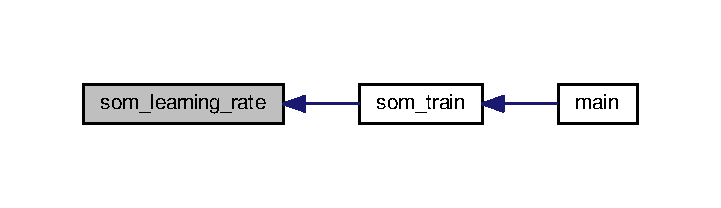
\includegraphics[width=346pt]{som_8c_ad269dc9f88dff13ec50497edc5bde2b0_icgraph}
\end{center}
\end{figure}


\hypertarget{som_8c_a1603f0fc083688b151b2ad414f9120a5}{\index{som.\-c@{som.\-c}!som\-\_\-neighbourhood@{som\-\_\-neighbourhood}}
\index{som\-\_\-neighbourhood@{som\-\_\-neighbourhood}!som.c@{som.\-c}}
\subsubsection[{som\-\_\-neighbourhood}]{\setlength{\rightskip}{0pt plus 5cm}static void som\-\_\-neighbourhood (
\begin{DoxyParamCaption}
\item[{float $\ast$}]{neigh, }
\item[{int}]{x, }
\item[{int}]{y, }
\item[{float}]{radius, }
\item[{int}]{width, }
\item[{int}]{height}
\end{DoxyParamCaption}
)\hspace{0.3cm}{\ttfamily [static]}}}\label{som_8c_a1603f0fc083688b151b2ad414f9120a5}
Compute the neighbors of a given point which are in a given radius.

Generates a mask with \mbox{[}0, 1\mbox{]} values to activate the inside of the 'radius' radius circle centered in (x, y).


\begin{DoxyParams}[1]{Parameters}
\mbox{\tt out}  & {\em neigh} & The resulting mask array. \\
\hline
\mbox{\tt in}  & {\em x} & The abscissae of the radius center. \\
\hline
\mbox{\tt in}  & {\em y} & The ordinates of the radius center. \\
\hline
\mbox{\tt in}  & {\em radius} & The neighbooring radius. \\
\hline
\mbox{\tt in}  & {\em width} & The width of the network. \\
\hline
\mbox{\tt in}  & {\em height} & The height of the network. \\
\hline
\end{DoxyParams}


Here is the call graph for this function\-:\nopagebreak
\begin{figure}[H]
\begin{center}
\leavevmode
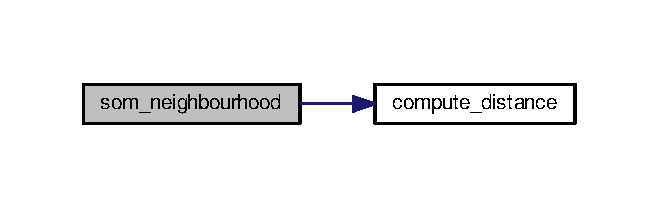
\includegraphics[width=316pt]{som_8c_a1603f0fc083688b151b2ad414f9120a5_cgraph}
\end{center}
\end{figure}




Here is the caller graph for this function\-:\nopagebreak
\begin{figure}[H]
\begin{center}
\leavevmode
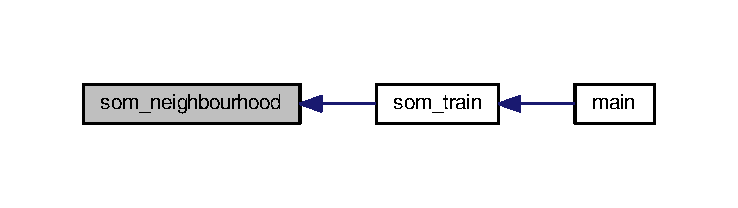
\includegraphics[width=350pt]{som_8c_a1603f0fc083688b151b2ad414f9120a5_icgraph}
\end{center}
\end{figure}


\hypertarget{som_8c_a3e18491e97ad6c14f54ba35aabfab994}{\index{som.\-c@{som.\-c}!som\-\_\-posterize@{som\-\_\-posterize}}
\index{som\-\_\-posterize@{som\-\_\-posterize}!som.c@{som.\-c}}
\subsubsection[{som\-\_\-posterize}]{\setlength{\rightskip}{0pt plus 5cm}void som\-\_\-posterize (
\begin{DoxyParamCaption}
\item[{float $\ast$$\ast$}]{post\-Pixels, }
\item[{float $\ast$$\ast$}]{orig\-Pixels, }
\item[{float $\ast$}]{train\mbox{[}$\,$\mbox{]}, }
\item[{unsigned int}]{nb\-Pixels, }
\item[{int}]{nb\-Neurons}
\end{DoxyParamCaption}
)}}\label{som_8c_a3e18491e97ad6c14f54ba35aabfab994}
Posterize an image from the trained S\-O\-M otput.

This function fill a vector containing the R\-G\-B values of each pixels of an image with the output of a trained S\-O\-M. The original image pixels R\-G\-B values are needed to compute the euclidian distance from its colors to the trained S\-I\-O\-M output colors. Basicaly you can see this function job as a smart color selector. For each pixel of the original image the function compute the \char`\"{}nearest\char`\"{} color among the reduced set of olors of the S\-O\-M output.


\begin{DoxyParams}[1]{Parameters}
\mbox{\tt out}  & {\em post\-Pixels} & The 2\-D array wich will contains the posterized pixels. \\
\hline
\mbox{\tt in}  & {\em orig\-Pixels} & The original image pixels. \\
\hline
\mbox{\tt in}  & {\em train} & The trained S\-O\-M output vector (its map). \\
\hline
\mbox{\tt in}  & {\em nb\-Pixels} & The number of pixels of th image (height $\ast$ width). \\
\hline
\mbox{\tt in}  & {\em nb\-Neurons} & The posterization level defined by its number of neurons. \\
\hline
\end{DoxyParams}


Here is the call graph for this function\-:\nopagebreak
\begin{figure}[H]
\begin{center}
\leavevmode
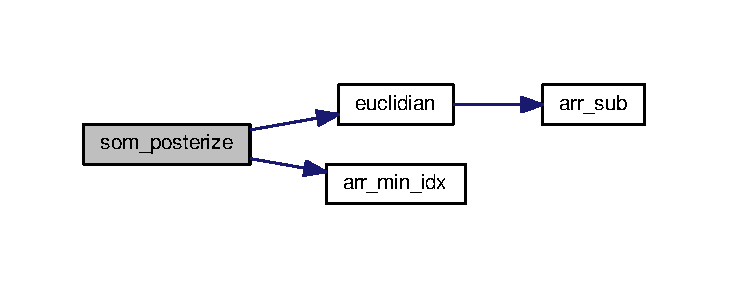
\includegraphics[width=350pt]{som_8c_a3e18491e97ad6c14f54ba35aabfab994_cgraph}
\end{center}
\end{figure}




Here is the caller graph for this function\-:\nopagebreak
\begin{figure}[H]
\begin{center}
\leavevmode
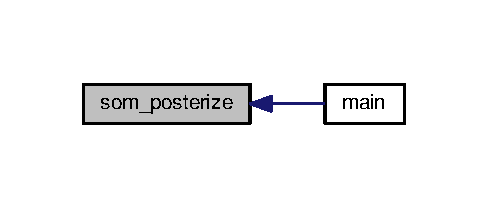
\includegraphics[width=234pt]{som_8c_a3e18491e97ad6c14f54ba35aabfab994_icgraph}
\end{center}
\end{figure}


\hypertarget{som_8c_a577de332dd926969d02e86228f65ad8f}{\index{som.\-c@{som.\-c}!som\-\_\-radius@{som\-\_\-radius}}
\index{som\-\_\-radius@{som\-\_\-radius}!som.c@{som.\-c}}
\subsubsection[{som\-\_\-radius}]{\setlength{\rightskip}{0pt plus 5cm}static float som\-\_\-radius (
\begin{DoxyParamCaption}
\item[{int}]{iter\-No, }
\item[{int}]{iter\-Count, }
\item[{int}]{width, }
\item[{int}]{height}
\end{DoxyParamCaption}
)\hspace{0.3cm}{\ttfamily [static]}}}\label{som_8c_a577de332dd926969d02e86228f65ad8f}
Compute and returns the neighbour radius value.

The radius is computed given the current iteration number, the maximum iteration number and the dimmensions of the network.


\begin{DoxyParams}[1]{Parameters}
\mbox{\tt in}  & {\em iter\-No} & The number of the current iteration. \\
\hline
\mbox{\tt in}  & {\em iter\-Count} & The maximum number of iterations. \\
\hline
\mbox{\tt in}  & {\em width} & The width of the network. \\
\hline
\mbox{\tt in}  & {\em height} & The height of the network.\\
\hline
\end{DoxyParams}
\begin{DoxyReturn}{Returns}
The computed radius. 
\end{DoxyReturn}


Here is the caller graph for this function\-:\nopagebreak
\begin{figure}[H]
\begin{center}
\leavevmode
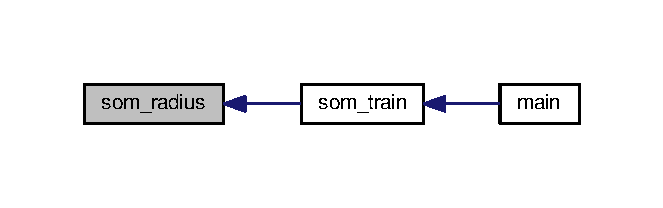
\includegraphics[width=318pt]{som_8c_a577de332dd926969d02e86228f65ad8f_icgraph}
\end{center}
\end{figure}


\hypertarget{som_8c_ab268269d2bda7d28482c0627e7c102ab}{\index{som.\-c@{som.\-c}!som\-\_\-train@{som\-\_\-train}}
\index{som\-\_\-train@{som\-\_\-train}!som.c@{som.\-c}}
\subsubsection[{som\-\_\-train}]{\setlength{\rightskip}{0pt plus 5cm}int som\-\_\-train (
\begin{DoxyParamCaption}
\item[{float $\ast$$\ast$}]{res, }
\item[{float $\ast$$\ast$}]{img\-Pixels, }
\item[{unsigned int}]{nb\-Pixels, }
\item[{int}]{nb\-Neurons, }
\item[{int}]{no\-Epoch, }
\item[{float}]{thresh}
\end{DoxyParamCaption}
)}}\label{som_8c_ab268269d2bda7d28482c0627e7c102ab}
Train the unsupervised S\-O\-M network.

The network is initialized with random (non-\/graduate) values. It is then trained with the image pixels (R\-G\-B). Once the network is done training the centroids of the resulting clusters is returned.

\begin{DoxyNote}{Note}
The length of the clusters depends on the parameter 'n'. The greatest n, the more colors in the clusters, the less posterized the image.
\end{DoxyNote}

\begin{DoxyParams}[1]{Parameters}
\mbox{\tt out}  & {\em res} & The resulting R, G and B clusters centroids. \\
\hline
\mbox{\tt in}  & {\em img\-Pixels} & The original image pixels. \\
\hline
\mbox{\tt in}  & {\em nb\-Pixels} & The number of pixels of th image (height $\ast$ width). \\
\hline
\mbox{\tt in}  & {\em nb\-Neurons} & The posterization leveldefined by its number of neurons. \\
\hline
\mbox{\tt in}  & {\em no\-Epoch} & Number of training passes (a too small number of epochs won't be enough for the network to correctly know the image but a too high value will force the network to modify the wieghts so much that the image can actually looks \char`\"{}ugly\char`\"{}). \\
\hline
\mbox{\tt in}  & {\em thresh} & The threshold value. The S\-O\-M delta parameter and the training rate are dicreasing from one epoch to the next. The treshold value set a stop condifition in case the value has fallen under this minimum value.\\
\hline
\end{DoxyParams}
\begin{DoxyReturn}{Returns}
S\-O\-M\-\_\-\-O\-K if everything goes right or S\-O\-M\-\_\-\-N\-O\-\_\-\-M\-E\-M\-O\-R\-Y if a memory allocation (malloc) fail. 
\end{DoxyReturn}


Here is the call graph for this function\-:\nopagebreak
\begin{figure}[H]
\begin{center}
\leavevmode
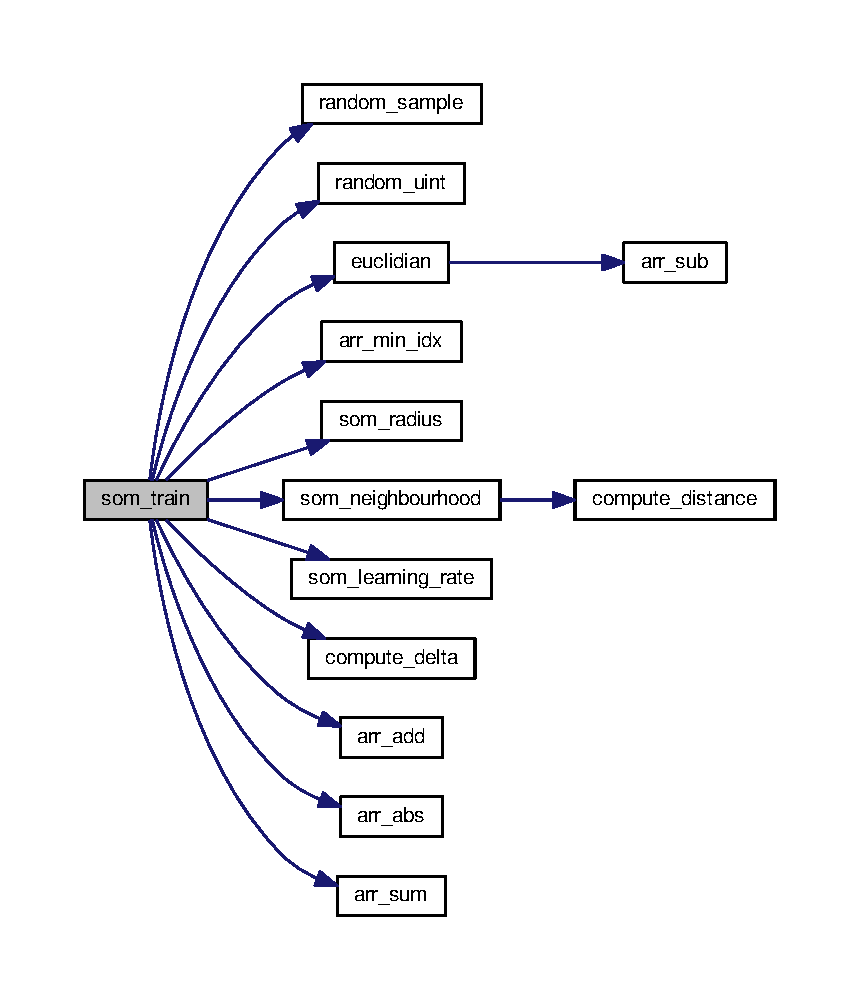
\includegraphics[width=350pt]{som_8c_ab268269d2bda7d28482c0627e7c102ab_cgraph}
\end{center}
\end{figure}




Here is the caller graph for this function\-:\nopagebreak
\begin{figure}[H]
\begin{center}
\leavevmode
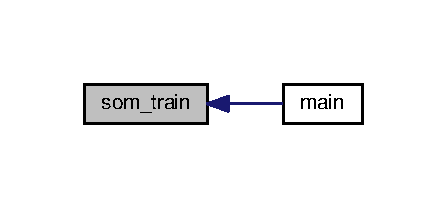
\includegraphics[width=214pt]{som_8c_ab268269d2bda7d28482c0627e7c102ab_icgraph}
\end{center}
\end{figure}



\hypertarget{som_8h}{\section{src/som.h File Reference}
\label{som_8h}\index{src/som.\-h@{src/som.\-h}}
}
{\ttfamily \#include $<$stdlib.\-h$>$}\\*
Include dependency graph for som.\-h\-:\nopagebreak
\begin{figure}[H]
\begin{center}
\leavevmode
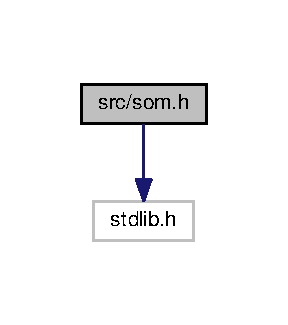
\includegraphics[width=138pt]{som_8h__incl}
\end{center}
\end{figure}
This graph shows which files directly or indirectly include this file\-:\nopagebreak
\begin{figure}[H]
\begin{center}
\leavevmode
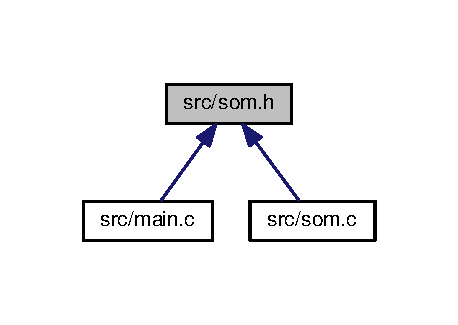
\includegraphics[width=220pt]{som_8h__dep__incl}
\end{center}
\end{figure}
\subsection*{Macros}
\begin{DoxyCompactItemize}
\item 
\#define \hyperlink{som_8h_ad2eb1fccbbafb6e5677c3d9ce2f5e0f7}{S\-O\-M\-\_\-\-N\-O\-\_\-\-M\-E\-M\-O\-R\-Y}~10
\item 
\#define \hyperlink{som_8h_a716494233ffdd2f324d12f608c0c03ae}{S\-O\-M\-\_\-\-O\-K}~0
\end{DoxyCompactItemize}
\subsection*{Functions}
\begin{DoxyCompactItemize}
\item 
void \hyperlink{som_8h_a392441531c1d2025232854783e7014bf}{compute\-\_\-delta} (float $\ast$res, float eta, float $\ast$neigh, size\-\_\-t nb\-Neigh, float chan, float $\ast$chan\-Arr)
\item 
int \hyperlink{som_8h_a0ef1fd049a245484d40c3ba9e5f8a636}{som\-\_\-train} (float $\ast$$\ast$res, float $\ast$$\ast$img\-Pixels, unsigned int nb\-Pixels, int nb\-Neurons, int no\-Epoch, float tresh)
\item 
void \hyperlink{som_8h_a3e18491e97ad6c14f54ba35aabfab994}{som\-\_\-posterize} (float $\ast$$\ast$post\-Pixels, float $\ast$$\ast$orig\-Pixels, float $\ast$train\mbox{[}$\,$\mbox{]}, unsigned int nb\-Pixels, int nb\-Neurons)
\end{DoxyCompactItemize}


\subsection{Macro Definition Documentation}
\hypertarget{som_8h_ad2eb1fccbbafb6e5677c3d9ce2f5e0f7}{\index{som.\-h@{som.\-h}!S\-O\-M\-\_\-\-N\-O\-\_\-\-M\-E\-M\-O\-R\-Y@{S\-O\-M\-\_\-\-N\-O\-\_\-\-M\-E\-M\-O\-R\-Y}}
\index{S\-O\-M\-\_\-\-N\-O\-\_\-\-M\-E\-M\-O\-R\-Y@{S\-O\-M\-\_\-\-N\-O\-\_\-\-M\-E\-M\-O\-R\-Y}!som.h@{som.\-h}}
\subsubsection[{S\-O\-M\-\_\-\-N\-O\-\_\-\-M\-E\-M\-O\-R\-Y}]{\setlength{\rightskip}{0pt plus 5cm}\#define S\-O\-M\-\_\-\-N\-O\-\_\-\-M\-E\-M\-O\-R\-Y~10}}\label{som_8h_ad2eb1fccbbafb6e5677c3d9ce2f5e0f7}
\hypertarget{som_8h_a716494233ffdd2f324d12f608c0c03ae}{\index{som.\-h@{som.\-h}!S\-O\-M\-\_\-\-O\-K@{S\-O\-M\-\_\-\-O\-K}}
\index{S\-O\-M\-\_\-\-O\-K@{S\-O\-M\-\_\-\-O\-K}!som.h@{som.\-h}}
\subsubsection[{S\-O\-M\-\_\-\-O\-K}]{\setlength{\rightskip}{0pt plus 5cm}\#define S\-O\-M\-\_\-\-O\-K~0}}\label{som_8h_a716494233ffdd2f324d12f608c0c03ae}


\subsection{Function Documentation}
\hypertarget{som_8h_a392441531c1d2025232854783e7014bf}{\index{som.\-h@{som.\-h}!compute\-\_\-delta@{compute\-\_\-delta}}
\index{compute\-\_\-delta@{compute\-\_\-delta}!som.h@{som.\-h}}
\subsubsection[{compute\-\_\-delta}]{\setlength{\rightskip}{0pt plus 5cm}void compute\-\_\-delta (
\begin{DoxyParamCaption}
\item[{float $\ast$}]{res, }
\item[{float}]{eta, }
\item[{float $\ast$}]{neigh, }
\item[{size\-\_\-t}]{nb\-Neigh, }
\item[{float}]{chan, }
\item[{float $\ast$}]{chan\-Arr}
\end{DoxyParamCaption}
)}}\label{som_8h_a392441531c1d2025232854783e7014bf}
Compute the new neurons values (learning stage).

This function compute the new neurons values depending on the learning rate (eta), the winner neighboors (neigh) and the choosed input vector (chan). The network wieght vectors inside the neighbooring radius are modified so that they will be more similar to the choosen input vector.


\begin{DoxyParams}[1]{Parameters}
\mbox{\tt out}  & {\em res} & The resulting array containing the delta values. \\
\hline
\mbox{\tt in}  & {\em eta} & The learning rate. \\
\hline
\mbox{\tt in}  & {\em neigh} & Array listing the current neighbors of the network. \\
\hline
\mbox{\tt in}  & {\em nb\-Neigh} & The size of the \char`\"{}neigh\char`\"{} array. \\
\hline
\mbox{\tt in}  & {\em chan} & The value of the color channel. \\
\hline
\mbox{\tt in}  & {\em chan\-Arr} & The array corresponding to the given channel. \\
\hline
\end{DoxyParams}


Here is the caller graph for this function\-:\nopagebreak
\begin{figure}[H]
\begin{center}
\leavevmode
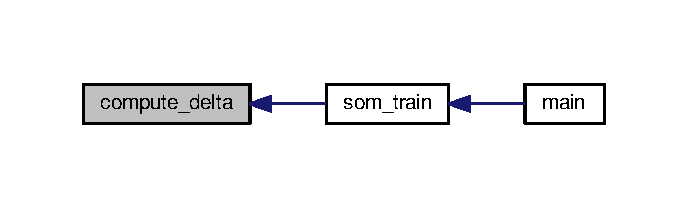
\includegraphics[width=330pt]{som_8h_a392441531c1d2025232854783e7014bf_icgraph}
\end{center}
\end{figure}


\hypertarget{som_8h_a3e18491e97ad6c14f54ba35aabfab994}{\index{som.\-h@{som.\-h}!som\-\_\-posterize@{som\-\_\-posterize}}
\index{som\-\_\-posterize@{som\-\_\-posterize}!som.h@{som.\-h}}
\subsubsection[{som\-\_\-posterize}]{\setlength{\rightskip}{0pt plus 5cm}void som\-\_\-posterize (
\begin{DoxyParamCaption}
\item[{float $\ast$$\ast$}]{post\-Pixels, }
\item[{float $\ast$$\ast$}]{orig\-Pixels, }
\item[{float $\ast$}]{train\mbox{[}$\,$\mbox{]}, }
\item[{unsigned int}]{nb\-Pixels, }
\item[{int}]{nb\-Neurons}
\end{DoxyParamCaption}
)}}\label{som_8h_a3e18491e97ad6c14f54ba35aabfab994}
Posterize an image from the trained S\-O\-M otput.

This function fill a vector containing the R\-G\-B values of each pixels of an image with the output of a trained S\-O\-M. The original image pixels R\-G\-B values are needed to compute the euclidian distance from its colors to the trained S\-I\-O\-M output colors. Basicaly you can see this function job as a smart color selector. For each pixel of the original image the function compute the \char`\"{}nearest\char`\"{} color among the reduced set of olors of the S\-O\-M output.


\begin{DoxyParams}[1]{Parameters}
\mbox{\tt out}  & {\em post\-Pixels} & The 2\-D array wich will contains the posterized pixels. \\
\hline
\mbox{\tt in}  & {\em orig\-Pixels} & The original image pixels. \\
\hline
\mbox{\tt in}  & {\em train} & The trained S\-O\-M output vector (its map). \\
\hline
\mbox{\tt in}  & {\em nb\-Pixels} & The number of pixels of th image (height $\ast$ width). \\
\hline
\mbox{\tt in}  & {\em nb\-Neurons} & The posterization level defined by its number of neurons. \\
\hline
\end{DoxyParams}


Here is the call graph for this function\-:\nopagebreak
\begin{figure}[H]
\begin{center}
\leavevmode
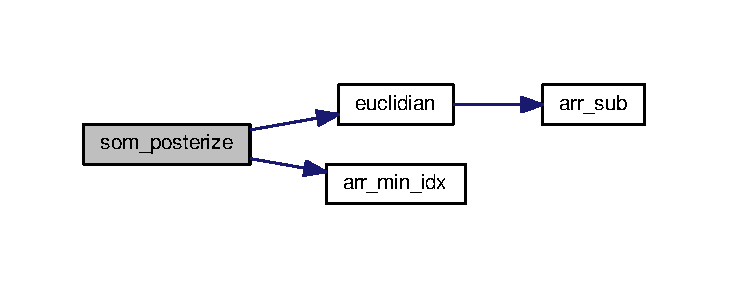
\includegraphics[width=350pt]{som_8h_a3e18491e97ad6c14f54ba35aabfab994_cgraph}
\end{center}
\end{figure}




Here is the caller graph for this function\-:\nopagebreak
\begin{figure}[H]
\begin{center}
\leavevmode
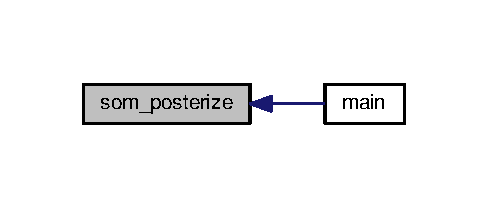
\includegraphics[width=234pt]{som_8h_a3e18491e97ad6c14f54ba35aabfab994_icgraph}
\end{center}
\end{figure}


\hypertarget{som_8h_a0ef1fd049a245484d40c3ba9e5f8a636}{\index{som.\-h@{som.\-h}!som\-\_\-train@{som\-\_\-train}}
\index{som\-\_\-train@{som\-\_\-train}!som.h@{som.\-h}}
\subsubsection[{som\-\_\-train}]{\setlength{\rightskip}{0pt plus 5cm}int som\-\_\-train (
\begin{DoxyParamCaption}
\item[{float $\ast$$\ast$}]{res, }
\item[{float $\ast$$\ast$}]{img\-Pixels, }
\item[{unsigned int}]{nb\-Pixels, }
\item[{int}]{nb\-Neurons, }
\item[{int}]{no\-Epoch, }
\item[{float}]{thresh}
\end{DoxyParamCaption}
)}}\label{som_8h_a0ef1fd049a245484d40c3ba9e5f8a636}
Train the unsupervised S\-O\-M network.

The network is initialized with random (non-\/graduate) values. It is then trained with the image pixels (R\-G\-B). Once the network is done training the centroids of the resulting clusters is returned.

\begin{DoxyNote}{Note}
The length of the clusters depends on the parameter 'n'. The greatest n, the more colors in the clusters, the less posterized the image.
\end{DoxyNote}

\begin{DoxyParams}[1]{Parameters}
\mbox{\tt out}  & {\em res} & The resulting R, G and B clusters centroids. \\
\hline
\mbox{\tt in}  & {\em img\-Pixels} & The original image pixels. \\
\hline
\mbox{\tt in}  & {\em nb\-Pixels} & The number of pixels of th image (height $\ast$ width). \\
\hline
\mbox{\tt in}  & {\em nb\-Neurons} & The posterization leveldefined by its number of neurons. \\
\hline
\mbox{\tt in}  & {\em no\-Epoch} & Number of training passes (a too small number of epochs won't be enough for the network to correctly know the image but a too high value will force the network to modify the wieghts so much that the image can actually looks \char`\"{}ugly\char`\"{}). \\
\hline
\mbox{\tt in}  & {\em thresh} & The threshold value. The S\-O\-M delta parameter and the training rate are dicreasing from one epoch to the next. The treshold value set a stop condifition in case the value has fallen under this minimum value.\\
\hline
\end{DoxyParams}
\begin{DoxyReturn}{Returns}
S\-O\-M\-\_\-\-O\-K if everything goes right or S\-O\-M\-\_\-\-N\-O\-\_\-\-M\-E\-M\-O\-R\-Y if a memory allocation (malloc) fail. 
\end{DoxyReturn}


Here is the call graph for this function\-:\nopagebreak
\begin{figure}[H]
\begin{center}
\leavevmode
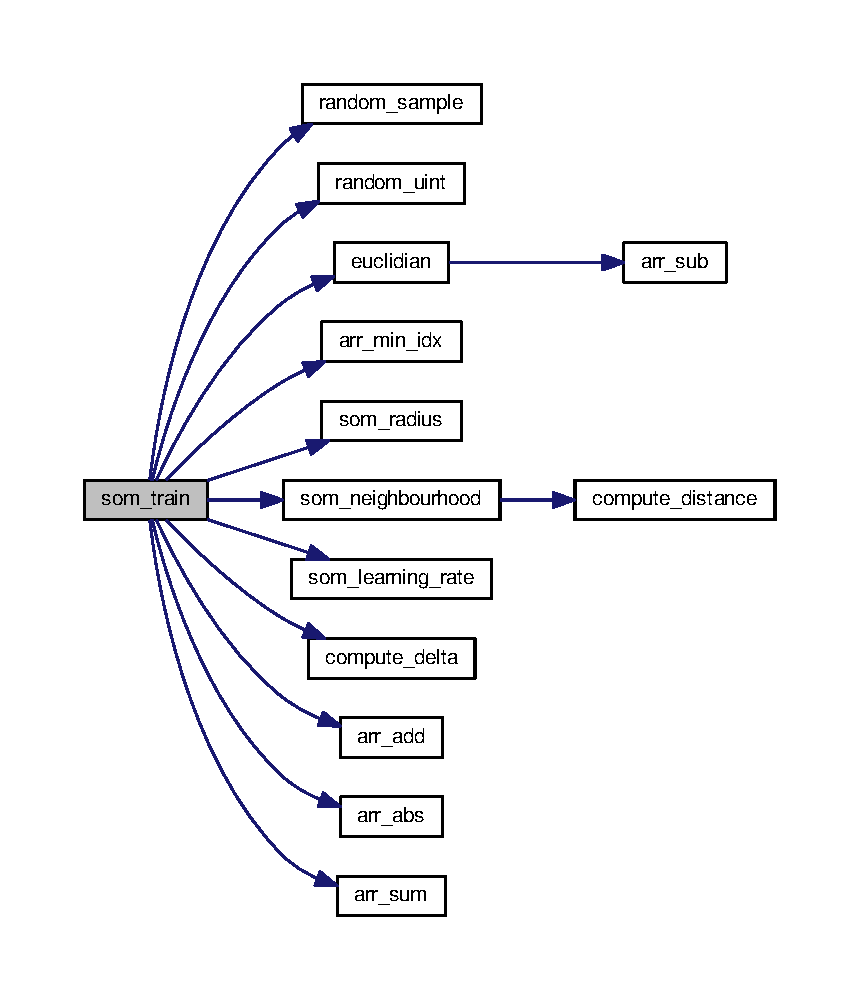
\includegraphics[width=350pt]{som_8h_a0ef1fd049a245484d40c3ba9e5f8a636_cgraph}
\end{center}
\end{figure}




Here is the caller graph for this function\-:\nopagebreak
\begin{figure}[H]
\begin{center}
\leavevmode
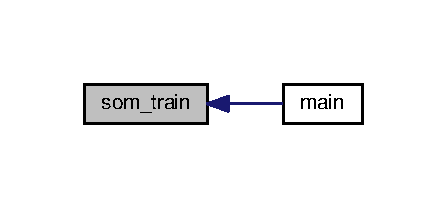
\includegraphics[width=214pt]{som_8h_a0ef1fd049a245484d40c3ba9e5f8a636_icgraph}
\end{center}
\end{figure}



\hypertarget{util_8c}{\section{src/util.c File Reference}
\label{util_8c}\index{src/util.\-c@{src/util.\-c}}
}


Contains helper functions use in any other source file.  


{\ttfamily \#include $<$stdlib.\-h$>$}\\*
{\ttfamily \#include \char`\"{}util.\-h\char`\"{}}\\*
{\ttfamily \#include \char`\"{}arr.\-h\char`\"{}}\\*
Include dependency graph for util.\-c\-:\nopagebreak
\begin{figure}[H]
\begin{center}
\leavevmode
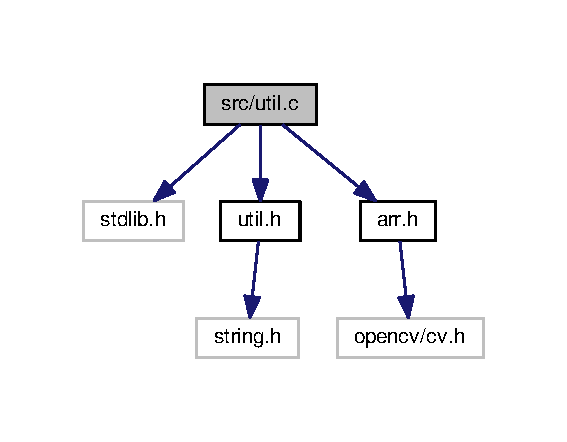
\includegraphics[width=272pt]{util_8c__incl}
\end{center}
\end{figure}
\subsection*{Functions}
\begin{DoxyCompactItemize}
\item 
void \hyperlink{util_8c_a92c1113e88f00f1fe38f88e29ea085e4}{random\-\_\-sample} (float $\ast$arr, size\-\_\-t size)
\item 
unsigned int \hyperlink{util_8c_afd86049c98dab897936e62cc9851a838}{random\-\_\-uint} (unsigned int \hyperlink{util_8h_affe776513b24d84b39af8ab0930fef7f}{max})
\item 
const char $\ast$ \hyperlink{util_8c_a06a7e80f6a756ec12b2ac12ea3d5f206}{get\-\_\-filename\-\_\-ext} (const char $\ast$filename)
\end{DoxyCompactItemize}


\subsection{Detailed Description}
Contains helper functions use in any other source file. \begin{DoxyAuthor}{Author}
Mathieu Fourcroy 
\end{DoxyAuthor}
\begin{DoxyDate}{Date}
07/15 
\end{DoxyDate}


\subsection{Function Documentation}
\hypertarget{util_8c_a06a7e80f6a756ec12b2ac12ea3d5f206}{\index{util.\-c@{util.\-c}!get\-\_\-filename\-\_\-ext@{get\-\_\-filename\-\_\-ext}}
\index{get\-\_\-filename\-\_\-ext@{get\-\_\-filename\-\_\-ext}!util.c@{util.\-c}}
\subsubsection[{get\-\_\-filename\-\_\-ext}]{\setlength{\rightskip}{0pt plus 5cm}const char$\ast$ get\-\_\-filename\-\_\-ext (
\begin{DoxyParamCaption}
\item[{const char $\ast$}]{filename}
\end{DoxyParamCaption}
)}}\label{util_8c_a06a7e80f6a756ec12b2ac12ea3d5f206}
Determine the extension (format) of a file.


\begin{DoxyParams}[1]{Parameters}
\mbox{\tt in}  & {\em filename} & The file name or its full path.\\
\hline
\end{DoxyParams}
\begin{DoxyReturn}{Returns}
The file extension (for instance jpg or png). 
\end{DoxyReturn}


Here is the caller graph for this function\-:\nopagebreak
\begin{figure}[H]
\begin{center}
\leavevmode
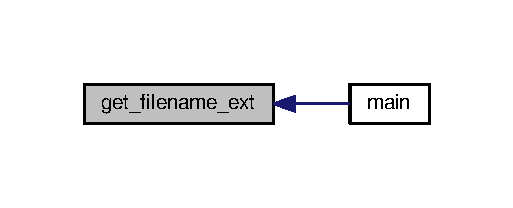
\includegraphics[width=246pt]{util_8c_a06a7e80f6a756ec12b2ac12ea3d5f206_icgraph}
\end{center}
\end{figure}


\hypertarget{util_8c_a92c1113e88f00f1fe38f88e29ea085e4}{\index{util.\-c@{util.\-c}!random\-\_\-sample@{random\-\_\-sample}}
\index{random\-\_\-sample@{random\-\_\-sample}!util.c@{util.\-c}}
\subsubsection[{random\-\_\-sample}]{\setlength{\rightskip}{0pt plus 5cm}void random\-\_\-sample (
\begin{DoxyParamCaption}
\item[{float $\ast$}]{arr, }
\item[{size\-\_\-t}]{size}
\end{DoxyParamCaption}
)}}\label{util_8c_a92c1113e88f00f1fe38f88e29ea085e4}
Fill the given array with float numbers between 0 and 1.

\begin{DoxyNote}{Note}
You must run srand() before in order to initialize the random number generation seed. 

The array 'arr' size must be 'size'.
\end{DoxyNote}

\begin{DoxyParams}[1]{Parameters}
\mbox{\tt out}  & {\em arr} & The array to fill. \\
\hline
\mbox{\tt in}  & {\em size} & The number of value to add to the array. \\
\hline
\end{DoxyParams}


Here is the caller graph for this function\-:\nopagebreak
\begin{figure}[H]
\begin{center}
\leavevmode
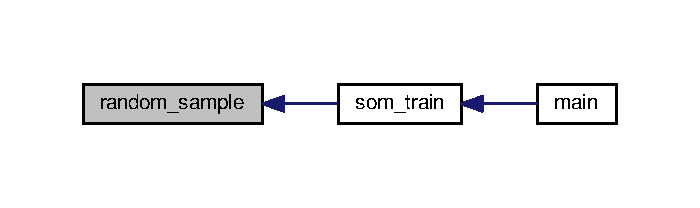
\includegraphics[width=336pt]{util_8c_a92c1113e88f00f1fe38f88e29ea085e4_icgraph}
\end{center}
\end{figure}


\hypertarget{util_8c_afd86049c98dab897936e62cc9851a838}{\index{util.\-c@{util.\-c}!random\-\_\-uint@{random\-\_\-uint}}
\index{random\-\_\-uint@{random\-\_\-uint}!util.c@{util.\-c}}
\subsubsection[{random\-\_\-uint}]{\setlength{\rightskip}{0pt plus 5cm}unsigned int random\-\_\-uint (
\begin{DoxyParamCaption}
\item[{unsigned int}]{max}
\end{DoxyParamCaption}
)}}\label{util_8c_afd86049c98dab897936e62cc9851a838}
Returns a randomly generated integer between 0 and the given maximum.


\begin{DoxyParams}[1]{Parameters}
\mbox{\tt in}  & {\em max} & The maximum boundary.\\
\hline
\end{DoxyParams}
\begin{DoxyReturn}{Returns}
The randomly generated number. 
\end{DoxyReturn}


Here is the caller graph for this function\-:\nopagebreak
\begin{figure}[H]
\begin{center}
\leavevmode
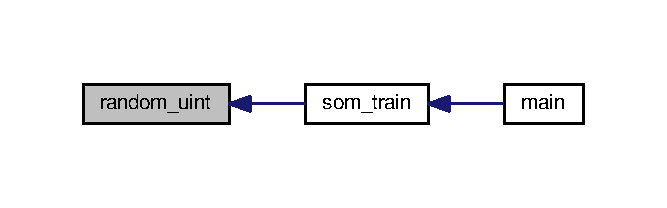
\includegraphics[width=320pt]{util_8c_afd86049c98dab897936e62cc9851a838_icgraph}
\end{center}
\end{figure}



\hypertarget{util_8h}{\section{src/util.h File Reference}
\label{util_8h}\index{src/util.\-h@{src/util.\-h}}
}
{\ttfamily \#include $<$string.\-h$>$}\\*
Include dependency graph for util.\-h\-:\nopagebreak
\begin{figure}[H]
\begin{center}
\leavevmode
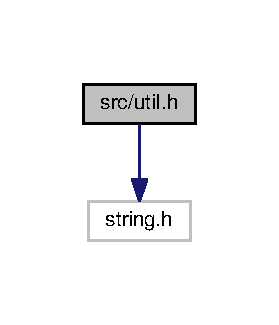
\includegraphics[width=134pt]{util_8h__incl}
\end{center}
\end{figure}
This graph shows which files directly or indirectly include this file\-:\nopagebreak
\begin{figure}[H]
\begin{center}
\leavevmode
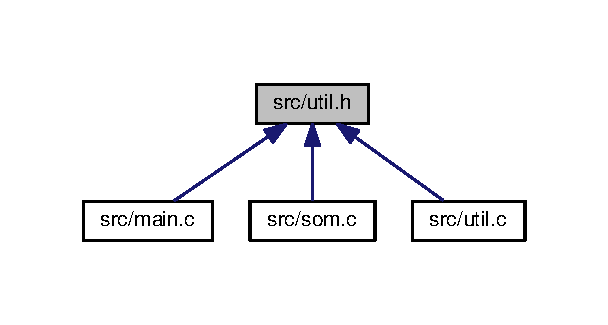
\includegraphics[width=292pt]{util_8h__dep__incl}
\end{center}
\end{figure}
\subsection*{Macros}
\begin{DoxyCompactItemize}
\item 
\#define \hyperlink{util_8h_affe776513b24d84b39af8ab0930fef7f}{max}(a, b)
\end{DoxyCompactItemize}
\subsection*{Functions}
\begin{DoxyCompactItemize}
\item 
void \hyperlink{util_8h_a92c1113e88f00f1fe38f88e29ea085e4}{random\-\_\-sample} (float $\ast$arr, size\-\_\-t size)
\item 
unsigned int \hyperlink{util_8h_afd86049c98dab897936e62cc9851a838}{random\-\_\-uint} (unsigned int \hyperlink{util_8h_affe776513b24d84b39af8ab0930fef7f}{max})
\item 
const char $\ast$ \hyperlink{util_8h_a06a7e80f6a756ec12b2ac12ea3d5f206}{get\-\_\-filename\-\_\-ext} (const char $\ast$filename)
\end{DoxyCompactItemize}


\subsection{Macro Definition Documentation}
\hypertarget{util_8h_affe776513b24d84b39af8ab0930fef7f}{\index{util.\-h@{util.\-h}!max@{max}}
\index{max@{max}!util.h@{util.\-h}}
\subsubsection[{max}]{\setlength{\rightskip}{0pt plus 5cm}\#define max(
\begin{DoxyParamCaption}
\item[{}]{a, }
\item[{}]{b}
\end{DoxyParamCaption}
)}}\label{util_8h_affe776513b24d84b39af8ab0930fef7f}
{\bfseries Value\-:}
\begin{DoxyCode}
(\{ \_\_typeof\_\_ (a) \_a = (a); \(\backslash\)
        \_\_typeof\_\_ (b) \_b = (b); \(\backslash\)
        \_a > \_b ? \_a : \_b; \})
\end{DoxyCode}


\subsection{Function Documentation}
\hypertarget{util_8h_a06a7e80f6a756ec12b2ac12ea3d5f206}{\index{util.\-h@{util.\-h}!get\-\_\-filename\-\_\-ext@{get\-\_\-filename\-\_\-ext}}
\index{get\-\_\-filename\-\_\-ext@{get\-\_\-filename\-\_\-ext}!util.h@{util.\-h}}
\subsubsection[{get\-\_\-filename\-\_\-ext}]{\setlength{\rightskip}{0pt plus 5cm}const char$\ast$ get\-\_\-filename\-\_\-ext (
\begin{DoxyParamCaption}
\item[{const char $\ast$}]{filename}
\end{DoxyParamCaption}
)}}\label{util_8h_a06a7e80f6a756ec12b2ac12ea3d5f206}
Determine the extension (format) of a file.


\begin{DoxyParams}[1]{Parameters}
\mbox{\tt in}  & {\em filename} & The file name or its full path.\\
\hline
\end{DoxyParams}
\begin{DoxyReturn}{Returns}
The file extension (for instance jpg or png). 
\end{DoxyReturn}


Here is the caller graph for this function\-:\nopagebreak
\begin{figure}[H]
\begin{center}
\leavevmode
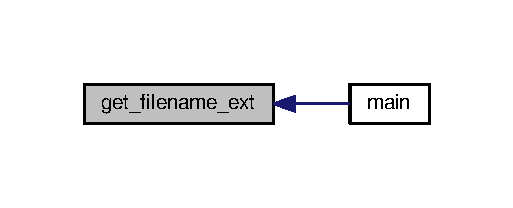
\includegraphics[width=246pt]{util_8h_a06a7e80f6a756ec12b2ac12ea3d5f206_icgraph}
\end{center}
\end{figure}


\hypertarget{util_8h_a92c1113e88f00f1fe38f88e29ea085e4}{\index{util.\-h@{util.\-h}!random\-\_\-sample@{random\-\_\-sample}}
\index{random\-\_\-sample@{random\-\_\-sample}!util.h@{util.\-h}}
\subsubsection[{random\-\_\-sample}]{\setlength{\rightskip}{0pt plus 5cm}void random\-\_\-sample (
\begin{DoxyParamCaption}
\item[{float $\ast$}]{arr, }
\item[{size\-\_\-t}]{size}
\end{DoxyParamCaption}
)}}\label{util_8h_a92c1113e88f00f1fe38f88e29ea085e4}
Fill the given array with float numbers between 0 and 1.

\begin{DoxyNote}{Note}
You must run srand() before in order to initialize the random number generation seed. 

The array 'arr' size must be 'size'.
\end{DoxyNote}

\begin{DoxyParams}[1]{Parameters}
\mbox{\tt out}  & {\em arr} & The array to fill. \\
\hline
\mbox{\tt in}  & {\em size} & The number of value to add to the array. \\
\hline
\end{DoxyParams}


Here is the caller graph for this function\-:\nopagebreak
\begin{figure}[H]
\begin{center}
\leavevmode
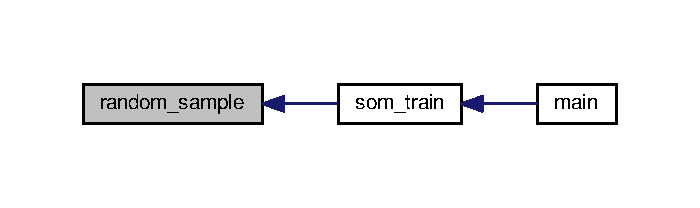
\includegraphics[width=336pt]{util_8h_a92c1113e88f00f1fe38f88e29ea085e4_icgraph}
\end{center}
\end{figure}


\hypertarget{util_8h_afd86049c98dab897936e62cc9851a838}{\index{util.\-h@{util.\-h}!random\-\_\-uint@{random\-\_\-uint}}
\index{random\-\_\-uint@{random\-\_\-uint}!util.h@{util.\-h}}
\subsubsection[{random\-\_\-uint}]{\setlength{\rightskip}{0pt plus 5cm}unsigned int random\-\_\-uint (
\begin{DoxyParamCaption}
\item[{unsigned int}]{max}
\end{DoxyParamCaption}
)}}\label{util_8h_afd86049c98dab897936e62cc9851a838}
Returns a randomly generated integer between 0 and the given maximum.


\begin{DoxyParams}[1]{Parameters}
\mbox{\tt in}  & {\em max} & The maximum boundary.\\
\hline
\end{DoxyParams}
\begin{DoxyReturn}{Returns}
The randomly generated number. 
\end{DoxyReturn}


Here is the caller graph for this function\-:\nopagebreak
\begin{figure}[H]
\begin{center}
\leavevmode
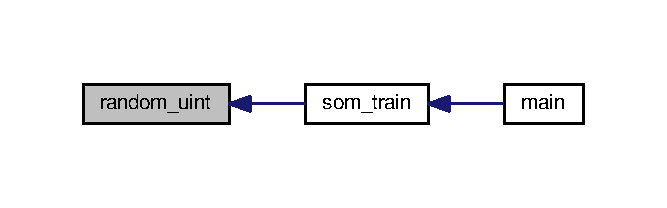
\includegraphics[width=320pt]{util_8h_afd86049c98dab897936e62cc9851a838_icgraph}
\end{center}
\end{figure}



%--- End generated contents ---

% Index
\newpage
\phantomsection
\addcontentsline{toc}{chapter}{Index}
\printindex

\end{document}
